\documentclass[10pt]{article}

\usepackage[margin=0.85in]{geometry}
\usepackage{amsmath,amssymb}
\usepackage{booktabs}
\usepackage{enumitem}
\usepackage{microtype}
\usepackage{multirow}
\usepackage{placeins}
\usepackage{xspace}
\usepackage{xcolor}
\usepackage{hyperref}
\usepackage{graphicx}
\usepackage{tikz}
\usepackage{pgfplots}
\usepgfplotslibrary{groupplots}
\usetikzlibrary{arrows.meta,positioning,fit,shapes.geometric}
\pgfplotsset{compat=1.18}

\hypersetup{
  colorlinks=true,
  linkcolor=blue!55!black,
  citecolor=green!35!black,
  urlcolor=blue!55!black
}
\setlist{leftmargin=*,nosep}
\newcommand{\system}{NaviSched\xspace}
\newcommand{\method}{CostScheduler\xspace}
\newcommand{\code}[1]{\texttt{#1}}
\newcommand{\keydata}[1]{\textcolor{green!40!black}{\textbf{#1}}}
\newcommand{\alertdata}[1]{\textcolor{red!70!black}{\textbf{#1}}}

\title{NaviSched: State-Aware Cost Optimization for\\
Distributed LLM Prefill Scheduling}
\author{zhang7\\
\href{mailto:zq103303@alibaba-inc.com}{\texttt{zq103303@alibaba-inc.com}}}
\date{}

\begin{document}
\maketitle

\begin{abstract}
Disaggregated large-language-model serving separates prompt processing
(prefill) from token generation, allowing the two phases to scale
independently. This separation creates a routing problem that conventional
load balancing does not solve: each prefill replica has a different prefix
cache, batching changes execution cost nonlinearly, queue state changes while
a decision is in flight, and maximizing cache hits alone can overload a small
set of replicas. We present \system, a distributed scheduling layer that
combines request features, exact prefix-cache metadata, queue state, and
online-fitted batch latency models in one closed control loop.

The central policy, \method, formulates a scheduling round as a continuous
request-to-node assignment. It predicts each candidate batch with a nonlinear
model, optimizes a latency/efficiency objective under one simplex constraint
per request, and converts the best projected solution into discrete routes.
We identify a dispersion failure in a direct linear latency weighting: deeper
optimization may fractionalize requests across more nodes even when the
eventual decision is discrete. A scaled logarithmic weighting penalizes such
dispersion while retaining a smooth analytic gradient. The implementation
executes node-wise forward/backward work and request-wise projection as an
alternating parallel dataflow graph, maintains cache and queue state beside
each model server, and confines diagnostic replay overhead to explicitly
sampled requests.

Trace-driven experiments exercise the same scheduling graph and state
protocol as deployment. They compare random, cache-greedy, and cost-aware
routing; sweep the online/offline tradeoff, optimization depth, and collection
window; and evaluate independent versus shared pools under heterogeneous
prompt distributions. On the single-workload trace, CostScheduler sustains
178.1 QPS at 363.3 ms mean and 426.2 ms P99 end-to-end latency, whereas random
and the NaviSched maximum-cache-hit proxy build 75.8 s and 87.3 s of mean
queue delay. A unified heterogeneous pool changes mean latency from 376.6 to
347.8 ms at equal aggregate capacity. These gains are not universal: larger
collection windows trade latency for batching, deeper optimization is worse
in the canonical loop-cap sweep, and near-one tradeoff weights sharply regress
latency and throughput. The results show why cache locality, batching,
queueing, prediction accuracy, and scheduler compute must be evaluated
together rather than as independent heuristics.
\end{abstract}

\section{Introduction}

An LLM request has two computationally different phases. Prefill processes
the input prompt and materializes key-value (KV) state; decode then generates
tokens autoregressively. Disaggregated serving places these phases on
different workers so that capacity can be assigned according to their
different resource and latency profiles~\cite{distserve,splitwise,mooncake}.
The prefill tier then requires a router to choose a worker for every prompt.

This choice is not ordinary least-connections routing. A worker that already
holds a long prefix can skip substantial computation. A lightly queued worker
may still be slower if it misses that prefix. Conversely, always selecting the
largest cache hit can concentrate traffic and destroy tail latency. The
execution time of several prompts batched together is not the sum of their
single-request times, and the best batch depends on each prompt's hit and miss
token counts. Finally, the router only observes distributed state after
communication and processing delays. A practical policy must make a joint
decision from imperfect but internally consistent state.

Existing model servers provide efficient paged KV memory, continuous
batching, and prefix reuse~\cite{vllm,orca,sglang}. These mechanisms operate
inside a replica. \system instead addresses the cluster-level question:
\emph{which prefill replica should receive each request, given the batches
that can be formed now and the work already queued at every replica?}

\system is designed as an additive layer. A request-side Client asks a Master
for a route; an Agent colocated with each prefill server reports cache and
execution facts. The Master batches scheduling requests and runs a replaceable
policy. The selected address returns to the existing router, which continues
to use the model framework's native request and streaming protocol. This
boundary avoids placing model traffic or KV contents on the control plane.

This paper makes four contributions:

\begin{itemize}
  \item It defines a state model and control loop that jointly exposes exact
        prefix-cache matches, queue work, execution state, and per-node
        latency models without synchronizing machine clocks.
  \item It presents a differentiable batch-assignment objective and a scaled
        logarithmic latency weight that makes the continuous relaxation agree
        more closely with its discrete routing outcome.
  \item It describes an implementation that alternates row-parallel gradient
        computation with column-parallel simplex projection, while retaining
        copy-on-write node snapshots and an explicitly sampled replay path.
  \item It evaluates policy, tradeoff, convergence, collection-window, and
        heterogeneous-pool behavior with deterministic trace replay and
        explicit scheduler-overhead measurements.
\end{itemize}

\section{Problem and Requirements}
\label{sec:problem}

\subsection{Prefill routing has coupled costs}

Let a scheduling round contain requests $i\in\mathcal{R}$ and ready prefill
nodes $n\in\mathcal{N}$. Request $i$ has $T_i$ prompt tokens and an ordered
sequence of full-block hashes. Node $n$ has a set of reusable hashes, queued
execution work, and a latency model fitted from batches it actually executed.
The common-prefix match determines hit tokens $H_{ni}$ and miss tokens
$M_{ni}=T_i-H_{ni}$.

A scheduler must account for four coupled effects:

\begin{enumerate}
  \item \textbf{Locality.} Larger $H_{ni}$ reduces prefill work, but the best
        cache location can change after insertion or eviction.
  \item \textbf{Batching.} A set of requests has one nonlinear batch cost.
        Summing independent request predictions is generally incorrect.
  \item \textbf{Queueing.} The new batch starts after already accepted work.
        Ignoring that work can repeatedly select the same apparently fast node.
  \item \textbf{Decision cost.} Scheduling itself is on the request path.
        A lower objective found too late may increase end-to-end latency.
\end{enumerate}

This coupling explains why a cache-greedy policy and a queue-greedy policy can
both fail. The former ignores contention; the latter can throw away useful KV
state and increase both compute and future queueing.

\subsection{System requirements}

The design follows six requirements. First, only nodes that completed a
handshake and supplied a valid model-server address may be scheduled. Second,
the Master must recover a complete cache view after restart or reconnection.
Third, queue estimates must derive from explicit batch lifecycle events rather
than wall-clock comparison across hosts. Fourth, policy extension must not
require changes to Client, Agent, or response construction. Fifth, detailed
diagnostics must be opt-in and must not delay unsampled requests. Sixth, adapters
must preserve each model framework's normal execution and cache semantics.

\section{Design Overview}
\label{sec:overview}

Figure~\ref{fig:architecture} shows the complete system. \system has three
roles, but only two control-plane paths. The request path carries a compact
description to the Master and returns one target. The state path carries
ordered Agent updates to the Master. Model requests and outputs remain on the
existing data path.

\begin{figure}[t]
\centering
\resizebox{\textwidth}{!}{%
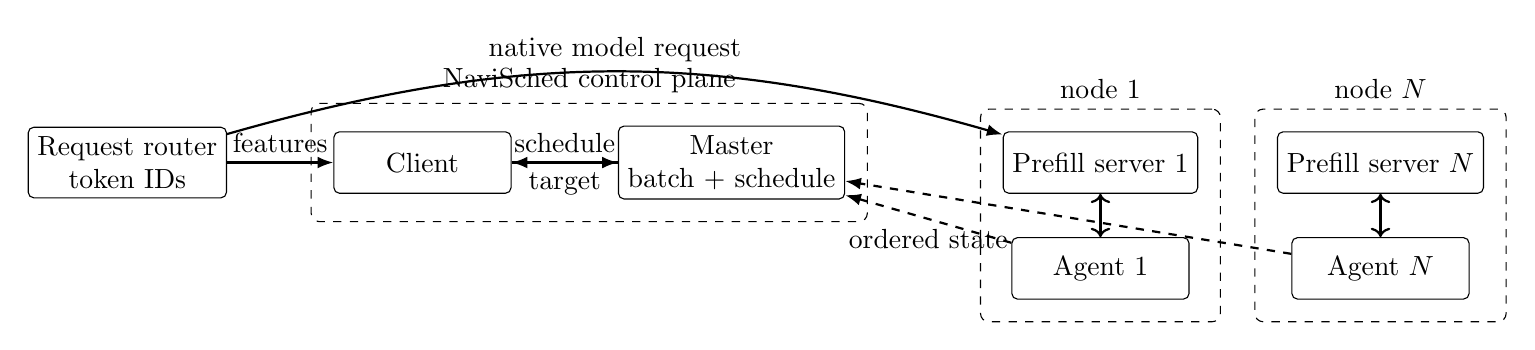
\begin{tikzpicture}[
  node distance=1.0cm and 1.35cm,
  box/.style={draw,rounded corners=2pt,minimum width=2.25cm,
              minimum height=0.78cm,align=center,fill=white},
  group/.style={draw,dashed,rounded corners=3pt,inner sep=8pt},
  flow/.style={-{Latex[length=2mm]},thick},
  state/.style={-{Latex[length=2mm]},thick,dashed}
]
  \node[box] (upstream) {Request router\\token IDs};
  \node[box,right=of upstream] (client) {Client};
  \node[box,right=of client,minimum width=2.7cm] (master)
      {Master\\batch + schedule};
  \node[box,right=2.0cm of master] (server1) {Prefill server 1};
  \node[box,below=0.55cm of server1] (agent1) {Agent 1};
  \node[box,right=1.0cm of server1] (servern) {Prefill server $N$};
  \node[box,below=0.55cm of servern] (agentn) {Agent $N$};

  \draw[flow] (upstream) -- node[above]{features} (client);
  \draw[flow] (client) -- node[above]{schedule} (master);
  \draw[flow] (master) -- node[below]{target} (client);
  \draw[flow,bend left=16] (upstream) to
      node[above]{native model request} (server1);
  \draw[state] (agent1) -- node[below]{ordered state} (master);
  \draw[state] (agentn) -- (master);
  \draw[flow,<->] (server1) -- (agent1);
  \draw[flow,<->] (servern) -- (agentn);

  \node[group,fit=(client)(master),label=above:{\system control plane}] {};
  \node[group,fit=(server1)(agent1),label=above:{node 1}] {};
  \node[group,fit=(servern)(agentn),label=above:{node $N$}] {};
\end{tikzpicture}
}
\caption{\system separates route decisions and state propagation from the
model framework's data path. The router sends the model request directly to
the selected prefill server.}
\label{fig:architecture}
\end{figure}

\paragraph{Client.}
The Client is embedded in a frontend or router after tokenization and before
prefill dispatch. It sends a request identifier, target service, token count,
block size, ordered block hashes, and timeout. It neither caches the cluster
view nor chooses a target.

\paragraph{Master.}
The Master owns the globally visible node state. It collects requests until a
count or time threshold, creates one immutable scheduling context for the
target service, invokes the configured policy, and converts each decision to
an address and batch identity. One Master can serve multiple target services;
each round sees the ready-node snapshot for exactly one service.

\paragraph{Agent.}
An Agent is colocated with one prefill executor and its KV cache. It observes
request acceptance, batch start and finish, actual hit/miss tokens, and cache
insertions or removals. It maintains local state needed both for immediate
prediction and for full recovery by a newly connected Master.

\subsection{One request from arrival to feedback}

Figure~\ref{fig:request-path} shows the causal loop. The upstream router has
already tokenized the prompt. It hashes only complete cache blocks with the
same algorithm and block size as the prefill runtime. The Master returns an
address; it does not proxy the request. At the selected node, the normal model
scheduler forms an execution batch. Agent instrumentation then reports actual
events, updating the state used by later decisions.

\begin{figure}[t]
\centering
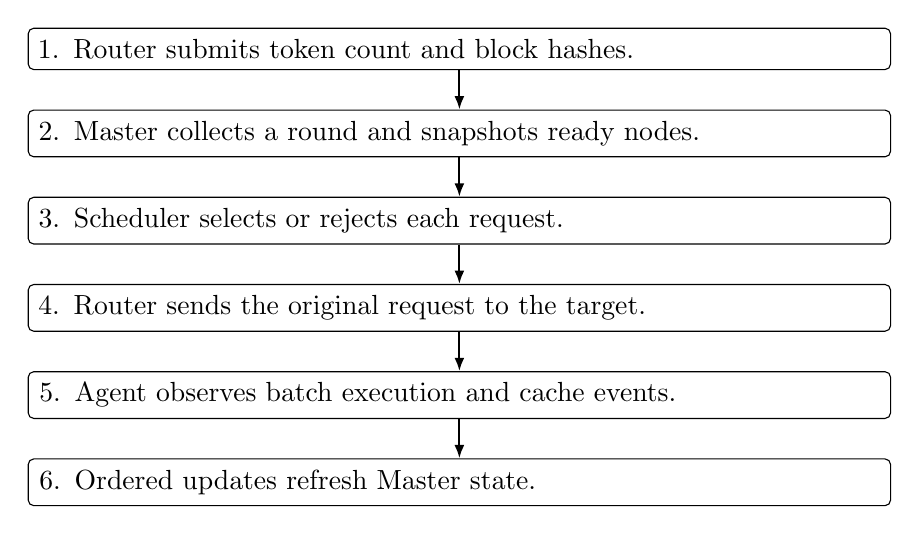
\begin{tikzpicture}[
  node distance=0.5cm,
  flowstep/.style={draw,rounded corners=2pt,align=left,
               text width=0.88\columnwidth,inner sep=4pt},
  arrow/.style={-{Latex[length=1.7mm]},thick}
]
  \node[flowstep] (a) {1. Router submits token count and block hashes.};
  \node[flowstep,below=of a] (b) {2. Master collects a round and snapshots ready nodes.};
  \node[flowstep,below=of b] (c) {3. Scheduler selects or rejects each request.};
  \node[flowstep,below=of c] (d) {4. Router sends the original request to the target.};
  \node[flowstep,below=of d] (e) {5. Agent observes batch execution and cache events.};
  \node[flowstep,below=of e] (f) {6. Ordered updates refresh Master state.};
  \draw[arrow] (a)--(b);
  \draw[arrow] (b)--(c);
  \draw[arrow] (c)--(d);
  \draw[arrow] (d)--(e);
  \draw[arrow] (e)--(f);
\end{tikzpicture}
\caption{A route closes the feedback loop only after the selected node
reports its resulting execution and cache state.}
\label{fig:request-path}
\end{figure}

Requests assigned to the same node in a round share a generated batch ID and
an expected size. The Agent tolerates partial arrival: it releases the batch
when all expected requests arrive or when its batch timer expires. This is
necessary because a successful Master decision does not guarantee that every
upstream request reaches the model server.

\section{Node State and Feedback}
\label{sec:state}

\subsection{Ready snapshots and ownership}

The Master separates nodes that are connecting from nodes eligible for
scheduling. A node enters a per-service ready map only after an online
handshake supplies a valid service address. Topology or stream termination
removes it from that map. A flat pending map remains available for observability
without exposing incomplete state to a scheduler.

Ready maps use copy-on-write replacement~\cite{copyonwrite}. Membership
changes are infrequent and copy a map; scheduling rounds retain shared node
objects from one snapshot and perform no membership lock acquisition while
evaluating candidates. Frequently changing fields use atomic counters or
small scoped locks, while related latency-model parameters are published as
one immutable snapshot so that a round never mixes revisions.

\subsection{Cache mirror and recovery}

For each Agent, both endpoints maintain a set of full-block hashes. Insert and
remove events update the Agent's local set and stream deltas to the Master. On
a new subscription, the Agent takes a locked full snapshot and sends it before
subsequent deltas. Thus a restarted Master reconstructs the same matching
state without requiring the model framework to replay cache initialization.
Only hashes and capacity metadata cross the control plane; token text and KV
tensors do not.

For request $i$, matching scans its ordered hashes until the first miss. If
$b_i$ is the request block size and $m_{ni}$ hashes match consecutively, then
$H_{ni}=b_i m_{ni}$. A partial final block has no hash and therefore cannot be
claimed as a cache hit. The Agent validates that reported actual hit tokens do
not exceed total tokens.

\subsection{Batch lifecycle and queue accounting}

The model adapter adds requests to the Agent's batching interface. When a
batch becomes ready, the callback receives a shared batch object and a finish
reporter. Starting the batch records its current requests and start time.
Finishing it supplies one actual request-stat record per request, including
the request ID, total tokens, and effective hit tokens.

The finish reporter is an RAII guard. If normal control flow omits completion,
its destructor closes the batch with an abnormal marker. The Agent accumulates
abnormal completion and timeout counters, publishes them, and includes them in
Master snapshots. This prevents one exceptional model path from leaving
permanent phantom work in the queue.

For every queued batch, the Agent predicts one execution duration. It keeps
the sum of predicted queued durations in an atomic integer: enqueue adds a
duration and completion subtracts it. Queue request counts are maintained
separately for snapshots. This makes an update $O(1)$ and avoids scanning or
copying all queued batches on every event. A query sees the queued sum plus
the remaining predicted time of the currently running batch.

Agent event timestamps are diagnostic labels only. \system does not compare
timestamps from different hosts or infer ordering from them. The report stream
preserves call order, and the Agent API requires lifecycle calls in order;
therefore the design does not assume synchronized clocks.

\section{Online Batch Latency Model}
\label{sec:model}

Each node fits its own model from completed physical batches. For request $i$
in an executed batch $\mathcal{A}$, let $H_i$ and $M_i$ be its actual cache-hit
and cache-miss counts. All hit/miss quantities in the model equations are
already expressed in 1K-token units, where one unit equals 1024 tokens; the
fixed scaling is applied before model evaluation and is therefore omitted
from the notation. Every quantity below is computed only from this same batch:
$B=|\mathcal{A}|$ is its request count; $R=\sum_iH_i$ and $C=\sum_iM_i$ are
its total hit and miss counts; and $C_2=\sum_iM_i^2$ and
$RC=\sum_iH_iM_i$ are batch sums, where every sum is over
$i\in\mathcal{A}$. The batch feature vector is
\begin{equation}
\mathbf{x}=
\left[1, B, R, C, C_2, RC\right].
\label{eq:features}
\end{equation}
Each node learns a nine-parameter vector
$\boldsymbol{\theta}=(\theta_0,\ldots,\theta_8)\in\mathbb{R}^9$.
Parameters $\theta_{0:5}$ are the six linear feature coefficients,
$\theta_6$ is the output offset, $\theta_7$ is the nonlinear output scale,
and $\theta_8$ is an additional score bias. The prediction first computes a
dimensionless linear score
\begin{equation}
z=\frac{\mathbf{x}^{\mathsf T}\boldsymbol{\theta}_{0:5}}{320}
  +\theta_8+1,
\end{equation}
Define the smooth rectifier $\phi(x)=x+\sqrt{x^2+4}$. The model then applies
the nonlinear output
\begin{equation}
F(\mathbf{x};\boldsymbol{\theta})=
\frac{\theta_6}{0.005}+
\frac{\theta_7}{0.02}\phi(z),
\label{eq:model}
\end{equation}
where $F$ is the predicted batch latency in milliseconds. The constants 320,
0.005, 0.02, and 1 are fixed numerical conditioning scales rather than learned
variables. The final transform behaves like a smooth rectifier while retaining
a finite, analytic gradient. Features include both aggregate work and the
distribution of miss tokens, allowing two batches with equal total tokens but
different request composition to have different predictions.

The Agent updates nine parameters with Adam~\cite{adam} on actual batch
latency. Parameters are installed as one revision and sent to the Master as a
unit. Cold-start fitting uses retained local history; inference and training
share Equation~\ref{eq:model}. During scheduling, the request-dependent part
of the linear score is precomputed once for every request-node pair, while the
nonlinear transform is evaluated once per candidate node and optimization
iteration.

\section{Cost-Aware Scheduling}
\label{sec:algorithm}

\subsection{Continuous assignment}

Directly searching $|\mathcal{N}|^{|\mathcal{R}|}$ assignments is infeasible,
where $|\cdot|$ denotes set cardinality. \method collects all relaxed
assignment weights in $W=[w_{ni}]$, with node row
$\mathbf{w}_n=(w_{ni})_{i\in\mathcal{R}}$. Each $w_{ni}\in[0,1]$ is the
fractional assignment of request $i$ to node $n$, with one simplex per request:
\begin{equation}
  \sum_{n\in\mathcal{N}} w_{ni}=1,\qquad w_{ni}\ge 0.
  \label{eq:simplex}
\end{equation}
For node $n$, let
$\boldsymbol{\theta}_n=(\theta_{n,0},\ldots,\theta_{n,8})$ be its current
latency-model parameters. Thus $\theta_{n,j}$ means parameter $j$ of node
$n$'s model; it is not a product of $\theta$ and $n$. Equation~\ref{eq:model}
uses $\boldsymbol{\theta}$ for one generic node, whereas scheduling evaluates
every candidate with its own $\boldsymbol{\theta}_n$. Using the hit and miss
counts $H_{ni}$ and $M_{ni}$ defined in Section~\ref{sec:problem}, request $i$
contributes
\begin{equation}
  c_{ni}=\theta_{n,1}
    +\theta_{n,2}H_{ni}
    +\theta_{n,3}M_{ni}
    +\theta_{n,4}M_{ni}^2
    +\theta_{n,5}H_{ni}M_{ni}
  \label{eq:request-cost}
\end{equation}
to the model's linear score. This is not a latency in milliseconds:
$\theta_{n,1}$ is the per-request-count contribution, the next two terms
represent hit and miss tokens, and the final two represent squared miss work
and the hit--miss interaction. The batch intercept $\theta_{n,0}$ is added
once in the following aggregate rather than once per request. The relaxed
aggregate score for node $n$ is
\begin{equation*}
\begin{aligned}
  z_n(\mathbf{w}_n)
    &=\frac{1}{320}\Biggl[\theta_{n,0}
      +\sum_{i\in\mathcal{R}}w_{ni}\Biggl(
        \theta_{n,1}
        +\theta_{n,2}H_{ni}
        +\theta_{n,3}M_{ni}
        \\[-0.1em]
    &\hspace{11.5em}
        +\theta_{n,4}M_{ni}^2
        +\theta_{n,5}H_{ni}M_{ni}
      \Biggr)\Biggr]+\theta_{n,8}+1.
\end{aligned}
\end{equation*}
The predicted batch latency is then
\begin{equation*}
  L_n(\mathbf{w}_n)
    =\frac{\theta_{n,6}}{0.005}
      +\frac{\theta_{n,7}}{0.02}
       \phi\!\left(z_n(\mathbf{w}_n)\right),
\end{equation*}
where $L_n$ is measured in milliseconds. Let $Q_n$ be the Agent's predicted
queue wait in milliseconds.

\subsection{Objective}

The optimized scalar objective uses
\begin{equation*}
  S_n=\sum_{i\in\mathcal{R}}w_{ni},
  \qquad
  U_n=\sum_{i\in\mathcal{R}}\frac{w_{ni}}{T_i},
\end{equation*}
where $S_n$ is the total request-assignment mass on node $n$, $U_n$ is its
token-normalized assignment mass, and $T_i$ is request $i$'s prompt-token
count. With these definitions, the objective is
\begin{equation}
\begin{aligned}
J(W)
  &=\frac{\lambda}{\sum_{i\in\mathcal{R}}T_i}
      \sum_{n\in\mathcal{N}}L_n(\mathbf{w}_n)S_n \\
  &\quad+\frac{1-\lambda}{|\mathcal{R}|}
      \sum_{n\in\mathcal{N}}
      \left(L_n(\mathbf{w}_n)+Q_n\right)g(U_n) \\[0.7em]
  &=\frac{\lambda}{\sum_{i\in\mathcal{R}}T_i}
    \sum_{n\in\mathcal{N}}
    \Biggl[\frac{\theta_{n,6}}{0.005}
      +\frac{\theta_{n,7}}{0.02}
       \phi\!\left(z_n(\mathbf{w}_n)\right)\Biggr]
    \sum_{i\in\mathcal{R}}w_{ni} \\[0.6em]
  &\quad+\frac{1-\lambda}{|\mathcal{R}|}
    \sum_{n\in\mathcal{N}}\Biggl\{
    \Biggl[\frac{\theta_{n,6}}{0.005}
      +\frac{\theta_{n,7}}{0.02}
       \phi\!\left(z_n(\mathbf{w}_n)\right)\Biggr]+Q_n\Biggr\}
      \frac{\log\!\Bigl(1+\kappa
        \sum_{i\in\mathcal{R}}w_{ni}/T_i\Bigr)}{\log\kappa}
    .
\end{aligned}
\label{eq:objective}
\end{equation}
The second equality performs a literal in-place substitution of $L_n$, $S_n$,
$U_n$, and $g$ without factoring, combining, or reordering the objective. The
nonlinear term remains $\phi(z_n(\mathbf{w}_n))$ to avoid repeating the full
node-score expression; that expression is given immediately before the
objective. The leading factors $\lambda$ and $1-\lambda$, both node sums, and
the original products remain in exactly the same positions as in the compact
form.
The concave weighting function is
\begin{equation}
  g(x)=\frac{\log(1+\kappa x)}{\log\kappa},\qquad \kappa=128.
\label{eq:concave}
\end{equation}
$\lambda\in[0,1]$ is the configured tradeoff weight, $x\geq 0$ is the generic
argument of $g$, and $\kappa=128$ tokens is a fixed concavity scale, making
$1+\kappa x$ dimensionless when $x=U_n$. All sums over $i$ and $n$ in
Equation~\ref{eq:objective} range over $\mathcal{R}$ and $\mathcal{N}$,
respectively. The first term approximates execution work per input token and favors
efficient batches. The second term approximates online latency while weighting
short requests more strongly through $1/T_i$. Thus low $\lambda$ emphasizes
interactive latency and high $\lambda$ emphasizes execution efficiency. The
parameter is a service-policy choice, not a statement that one operating point
dominates all workloads.

\subsection{Why the latency weight is concave}

An earlier objective used $g(x)=x$. Its continuous optimum could spread small
fractions of every request over many nodes. The final route takes only the
largest weight, so this fractional dilution did not correspond to a realizable
batch. More optimization could therefore reduce the continuous objective yet
produce smaller discrete batches and longer queues.

Equation~\ref{eq:concave} is increasing, smooth, and concave, with
\begin{equation}
  g'(x)=\frac{\kappa}{(1+\kappa x)\log\kappa}.
\end{equation}
For a fixed assignment mass, splitting it among additional nodes increases
the sum of a concave function with $g(0)=0$. The objective therefore charges
dispersion without adding a separate regularizer with incompatible units.
The scale $\kappa=128$ was selected by a fixed-context sweep: weaker curvature
retained dispersion, while much stronger curvature formed fewer batches but
increased execution and queue cost.

\subsection{Projected optimization}

Weights start from positive pseudo-random values normalized independently for
each request, producing $W^{(0)}$. At iteration $k\geq 0$, the optimizer uses
step size $\alpha_k>0$ and performs
\begin{align}
  \widetilde{W}^{(k+1)}
    &=W^{(k)}-\alpha_k\nabla_W J(W^{(k)}),\\
  W^{(k+1)}
    &=\Pi_{\Delta}\!\left(\widetilde{W}^{(k+1)}\right),
\end{align}
where $\widetilde{W}^{(k+1)}$ is the unconstrained update,
$\nabla_W J$ is the gradient with respect to all entries of $W$, and
$\Pi_{\Delta}$ projects every request column onto
$\Delta=\{\mathbf{v}\mid v_n\geq0,\sum_n v_n=1\}$, the probability
simplex~\cite{projectedsimplex}. The step size may decay but never below a
configured floor. After projection, $n_i=\arg\max_n w_{ni}$ is the candidate
discrete destination for request $i$. The optimizer retains the candidate
associated with the best observed projected objective, so a later step cannot
overwrite a better earlier solution.

Optimization runs at least the configured minimum and stops at either its loop
cap or a scheduling-time budget derived from the request collection window.
The actual loop count and stop reason are reported. This distinction matters:
a configured cap does not imply that every scheduling round executes that
many iterations.

\subsection{Complexity and parallel dataflow}

One iteration is $O(|\mathcal{R}||\mathcal{N}|)$ in work and the dense cost,
weight, and gradient matrices use the same asymptotic memory. The matrices are
node-major because model evaluation and backward propagation consume complete
node rows. Projection traverses request columns and uses bounded request tiles
to control workspace size.

The production scheduler is a dataflow graph, shown in
Figure~\ref{fig:optimizer-graph}. Preparation and forward/backward work are
partitioned by node. A barrier then releases projection workers partitioned by
request. A second barrier either starts another iteration or releases a final
row evaluation and result stage. Required edges provide stage synchronization;
the policy code does not implement its own thread pool.

\begin{figure}[t]
\centering
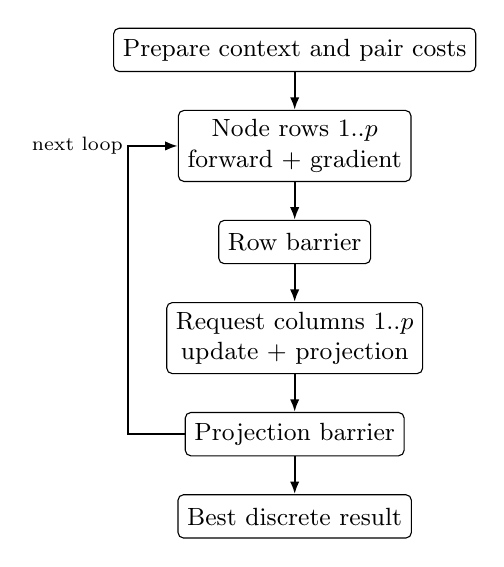
\begin{tikzpicture}[
  node distance=0.48cm and 0.35cm,
  box/.style={draw,rounded corners=2pt,align=center,
              minimum height=0.55cm,font=\small},
  arrow/.style={-{Latex[length=1.6mm]},thick}
]
  \node[box] (prep) {Prepare context and pair costs};
  \node[box,below=of prep] (r1) {Node rows 1..$p$\\forward + gradient};
  \node[box,below=of r1] (rb) {Row barrier};
  \node[box,below=of rb] (proj) {Request columns 1..$p$\\update + projection};
  \node[box,below=of proj] (pb) {Projection barrier};
  \node[box,below=of pb] (done) {Best discrete result};
  \draw[arrow] (prep)--(r1);
  \draw[arrow] (r1)--(rb);
  \draw[arrow] (rb)--(proj);
  \draw[arrow] (proj)--(pb);
  \draw[arrow] (pb.west) -- ++(-0.72cm,0) |-
      node[pos=0.5,left,fill=white,inner sep=1.5pt,font=\scriptsize]
      {next loop} (r1.west);
  \draw[arrow] (pb)--(done);
\end{tikzpicture}
\caption{Alternating node-row and request-column phases preserve the natural
access pattern of gradient evaluation and simplex projection.}
\label{fig:optimizer-graph}
\end{figure}

The hot path uses an analytic vector-Jacobian product. It evaluates the
nonlinear model and its scalar derivative once per node, then applies that
derivative to the precomputed pair costs. Automatic differentiation remains a
reference implementation for gradient tests, not a per-pair production tape.
This removes graph-node allocation and repeated nonlinear evaluation from the
$|\mathcal{R}||\mathcal{N}|$ loop.

\section{Engineering the Control Plane}
\label{sec:implementation}

\subsection{Scheduling contexts and policy extension}

A scheduling context is the sole object passed through a policy graph. It
contains one service's requests, immutable node handles, cache-match access,
and result slots. Match counts are computed when a policy requests them; a
policy that does not inspect cache pays no match cost. A synchronous policy
implements one scheduler kernel and calls either \code{selectNode} or
\code{reject} for every request. A staged policy can build a graph such as
Figure~\ref{fig:optimizer-graph} around the same context. Batch IDs, response
construction, timeout handling, and replay branching remain framework duties,
not extension APIs.

The implementation includes random routing as a topology-only baseline and
maximum-cache-hit routing as a cache-only baseline. Both are production
policies and examples of the extension surface; neither has special test-only
ordering in its decision path.

\subsection{Result path and replay path}

After scheduling, one result stage validates that every request has either a
selection or a rejection, assigns batch metadata, and emits independent Client
responses. When replay collection is enabled, the scheduler's context output
is branched in the Client graph. Responses without replay data are completed
first. An explicitly sampled response also carries the replay snapshot, and
its serialization and Client-side storage can delay that sampled request.
Production performance runs therefore disable replay collection; diagnostic
comparisons either report this perturbation or use the same sampling policy on
every compared configuration.

A replay records requests, node state, queue values, latency parameters,
cache-match counts, decisions, and scheduler-specific nested JSON. Offline
execution reconstructs fake node and cache objects and invokes the same policy
entry point. It does not change the production node-map layout or precompute
policy-specific fields. CostScheduler replay additionally records projected
loss, gradients, weights, loop count, stop reason, and stage timing. This makes
an individual decision inspectable while preserving the online code shape.

\subsection{Framework adapters}

Adapters are deliberately placed in the \system package. A model framework
needs only narrow lifecycle hooks. On the request side, an adapter receives
token IDs from the existing upstream tokenizer, computes the model-compatible
chained block hashes, invokes the Client, and passes the original request to
the selected endpoint through the existing transport. On the prefill side, an
observer maps the framework's real batch and KV events to Agent calls.

For a vLLM integration, only complete blocks are hashed and the parent hash
retains its full digest before a 64-bit wire representation is derived. The
effective block size must match the runtime cache configuration. Chunked
prefill reports only the tokens actually scheduled in that physical batch;
already computed prompt tokens count as reuse. Unsupported hash inputs, such
as unmodeled multimodal keys, are rejected rather than routed with a false
cache estimate. The integration is explicitly enabled, leaving the original
router and model-server paths unchanged when disabled.

\subsection{Failure behavior}

Topology refresh creates collectors for newly visible Agents. A failed or
terminated collector is retried at low frequency; healthy streams are not
rebuilt periodically. If a graph timer can no longer be refreshed, the graph
is already ending, so its external pipe is terminated. Subsequent producers
receive an error instead of blocking indefinitely.

Master restart is handled by Agent full snapshots followed by ordered deltas.
Agent shutdown first stops new work, drains or aborts owned batches, and closes
report streams. These mechanisms provide state recovery, not durable request
execution: the upstream serving layer remains responsible for retrying a
request whose scheduling or model RPC fails.

\section{Evaluation}
\label{sec:evaluation}

We ask five questions:

\begin{enumerate}
  \item How does joint cost optimization compare with random and cache-only
        routing?
  \item Does the concave latency weight correct the dispersion failure?
  \item How do $\lambda$, loop count, and collection window affect latency,
        cache reuse, utilization, and scheduler cost?
  \item Does one shared heterogeneous pool preserve short-request latency and
        improve capacity relative to workload-specific pools?
  \item Does scheduler computation remain small enough for the intended
        request and node scale?
\end{enumerate}

\subsection{Methodology}

The trace-driven simulator uses the production Client, Master scheduler graph,
Agent report protocol, cache matching, and latency model. It replaces only the
GPU executor with a deterministic logical executor. Agents form batches,
execute them sequentially, insert and evict cache blocks, and report actual
events through the same interfaces. Random seed is fixed to one and execution
noise has a 1\% standard-deviation ratio.

Replay Clients issue requests asynchronously at their recorded arrival-time
offsets; sending a request does not wait for earlier simulated execution to
finish. Each request follows the production Client-to-Master graph, where the
Master collects a scheduling window, snapshots ready Agents, and returns a
target and batch identity. The request is then forwarded to the selected
simulated Agent, which forms the assigned batches and executes one batch at a
time. The logical executor computes batch duration from a fixed nonlinear
latency function over prompt work and current cache hits, adds seeded noise,
and waits for that logical duration. On completion it updates the Agent's LRU
cache and emits the normal batch-finish and request-completion events. These
events update Master-visible state and the online latency model, while the
response closes the request graph and contributes batching, queueing,
execution, and end-to-end latency to the report.

The canonical single-workload experiment replays 53,751 requests over 300
logical seconds with 40 Agents and 10 Clients. The heterogeneous experiment
combines five 300-second middle trace segments, totaling 90,291 requests. Its
independent deployment uses per-workload pools of 33, 41, 9, 17, and 54 Agents
(154 total); the unified deployment gives the same requests access to one
154-Agent pool. Unless a sweep states otherwise, the Master collects at most
30 requests or waits 30 ms. Cache capacity is 300 GiB in aggregate.

All reported latency is uncompressed logical time. The final canonical suite
uses time-compression factor one, waits for all Agents to become ready, and
validates request count, Agent count, scheduler configuration, loop samples,
and completion. ``Utilization'' is logical executor busy time divided by
logical elapsed time. It measures occupied prefill capacity in this simulator;
it is not a hardware GPU utilization counter. Completion QPS includes replay
duration and drain time. Scheduler latency is measured inside the Master
scheduler graph and excludes collection wait, RPC, and model execution.

Experiments run on a dual-socket Intel Xeon Platinum 8469C host with 96
physical cores (192 hardware threads) and 1 TiB of memory. The binaries use an
optimized Clang build. CostScheduler uses an explicit parallelism of ten
workers. Single-workload and collection-window runs use initial step size 512;
heterogeneous-pool runs use 128. Step decay is disabled. The standard loop cap
is 50, while the collection-window sweep allows up to 200 iterations and still
obeys its per-round time budget.

The canonical launch configuration uses a latency-fit batch size of 100,000,
fit interval zero, learning rate 0.022, and no warmup samples. An interval of
zero delegates the trigger threshold to the fit batch size. No Agent reaches
100,000 completed physical batches in these runs, so online fitting is not
triggered and the default static model remains active. The report records both
launch configuration and runtime effective scheduler configuration. Every
canonical summary has zero unmatched batches. Table~\ref{tab:canonical-prediction}
therefore separates scheduler completion from prediction quality: the routes
and lifecycle accounting pass, but the heterogeneous default-model prediction
error is not a steady-state accuracy result.

\subsection{Objective correction and convergence}

The controlled objective ablation uses the same 60-second trace prefix, 40
Agents, 10 Clients, random seed, and 105 sampled scheduling contexts in every
run. Table~\ref{tab:objective-ablation} compares the old linear latency weight
with Equation~\ref{eq:concave}. Under the old objective,
increasing from two to 50 loops lowers predicted execution work but fragments
batches: mean queue delay rises from 3.23 to 24.14 ms and end-to-end latency
rises from 355.89 to 376.55 ms. With the scaled logarithm, deeper optimization
monotonically lowers queue-plus-execution cost from 330.76 ms at two loops to
326.84 ms at 50 loops. End-to-end latency is best at five loops (349.01 ms)
because later loops save model work but add scheduling time. This separates
objective quality from optimizer overhead: the projected objective improves,
but the route arrives later.

At 50 loops and $\lambda=0.1$, the correction reduces mean queue delay from
23.82 to 0.21 ms and P99 end-to-end latency from 600.97 to 392.73 ms. At
$\lambda=0.5$, it reduces queue delay from 60.21 to 0.97 ms and P99 from
711.75 to 409.52 ms. The consistent direction at multiple tradeoff settings
supports the dispersion diagnosis rather than a one-point tuning effect.

\subsection{Policy and tradeoff results}

Table~\ref{tab:strategy-baseline} compares the three policies on one trace.
At $\lambda=0.5$, CostScheduler completes the offered load at 178.1 QPS
with 363.3 ms mean and 426.2 ms P99 end-to-end latency. Random routing
reaches 113.8 QPS but accumulates 75.8 s of mean queue delay, while the
NaviSched maximum-cache-hit proxy reaches only 56.3 QPS despite increasing
the cache-hit rate from 13.0\% to 43.7\%. CostScheduler instead obtains a
31.2\% hit rate
without concentrating enough work to create the same queue. This comparison
is one deterministic trace replay rather than a confidence interval, but it
shows why cache locality alone is not a sufficient routing objective.
The maximum-cache-hit row is a NaviSched cache-only proxy and must not be read
as a measurement of the production FlexLB implementation.

Figure~\ref{fig:lambda-sweep} and Tables~\ref{tab:single-lambda},
\ref{tab:independent-lambda}, and~\ref{tab:unified-lambda} report the sampled
$\lambda$ sweep. The intended online region is near the low end of the range;
values close to one model an efficiency-oriented offline objective and should
not be interpreted as an online default. We retain the near-one samples
because they reveal when ignoring queue cost concentrates traffic.
The sweep does not improve every configuration. The single-workload results
are nearly flat from $\lambda=0$ through 0.25, then gradually degrade after
0.5 and accelerate near one: mean latency is 362.7 ms at zero, 363.3 ms at
0.5, 379.1 ms at 0.95, and 80.1 s at one. The unified pool is stable over a
wider low-to-mid range: mean latency is 347.8 ms at zero, 351.4 ms at 0.99,
and 374.8 ms at 0.999. At the pure $\lambda=1$ boundary it reaches 1.75 s mean
and 33.1 s P99 latency at 217.9 QPS. These boundary results are evidence for
operating-region selection, not a reason to report one universally dominant
parameter.

The tables report actual average loop count in addition to the configured cap.
When a time budget terminates optimization, these differ. This is essential
for interpreting apparent improvements at a higher cap: they may come from a
different number of completed loops or from a different scheduling delay.
Table~\ref{tab:loss-distribution} reports one objective value per scheduling
round, deduplicated by Master schedule ID. Since $\lambda$ changes the
objective itself, absolute loss is used only to compare optimization under the
same workload and $\lambda$, not to rank different tradeoff settings.

\subsection{Heterogeneous sharing, window, and capacity}

Table~\ref{tab:pool-baseline} compares independent and unified deployment at
equal aggregate node count. The sampled sweeps in
Tables~\ref{tab:independent-lambda} and~\ref{tab:unified-lambda} retain metrics
for each source trace after mixing, so a favorable aggregate cannot hide a
long-prompt workload delaying short prompts. The capacity experiment then
reduces the shared pool from 154 to 145 Agents while holding the request set
fixed.

At $\lambda=0$, replacing five independent pools with one 154-Agent pool
reduces mean end-to-end latency from 376.6 to 347.8 ms and P99 from 835.9 to
412.1 ms, while completion throughput remains near 299 QPS. Reducing the
shared pool to 145 Agents produces 347.8 ms mean and 411.5 ms P99 at 299.0
QPS. This deterministic trace therefore shows no degradation from the 5.8\%
node-count reduction, but it does not establish a general capacity saving or
justify extrapolation to another workload mix.

Table~\ref{tab:window-sweep} varies both the collection limit and wait window
from 30 to 100. Larger windows expose more joint assignment opportunities but
directly add collection delay and enlarge the dense optimization matrix. Mean
batch size rises from 2.136 to 2.648 and card-time falls from 8401.8 to
6702.5 s, while mean latency rises from 378.5 to 403.3 ms and P99 from 436.6
to 486.9 ms. This is a batching-versus-latency tradeoff, not a uniform gain.
Table~\ref{tab:loop-sweep} isolates the loop cap on the shared workload. These
experiments jointly show that batch opportunity and optimization depth must be
budgeted against time on the request path, rather than maximized independently.
Increasing the cap from two to 50 raises mean end-to-end latency from 339.2
to 347.8 ms and P99 from 408.0 to 412.1 ms, while mean scheduler time rises
from 0.565 to 7.516 ms. Ten loops produce 341.9 ms mean latency. In this
canonical trace deeper optimization does not improve the service outcome;
this observation is scoped to the measured trace rather than asserted as a
general property of the optimizer.

\subsection{Scheduler scalability}

The dense relaxation deliberately pays $O(RN)$ to compare every request-node
pair. Row/column parallelism removes compute bottlenecks until matrix traffic
approaches memory-bandwidth limits. Analytic gradients avoid an automatic-
differentiation object per pair; preparation caches pair costs; update and
simplex projection share one traversal; and bounded tiles avoid a full
transposed matrix. For large deployments, the scheduler's practical capacity
therefore depends on request-window size, candidate-node count, memory
bandwidth, and the time budget together. Candidate filtering or sparse
optimization is future work rather than hidden behavior in the current
results.

% Generated by generate_artifacts.py; do not edit.
\begin{figure*}[t]
\centering
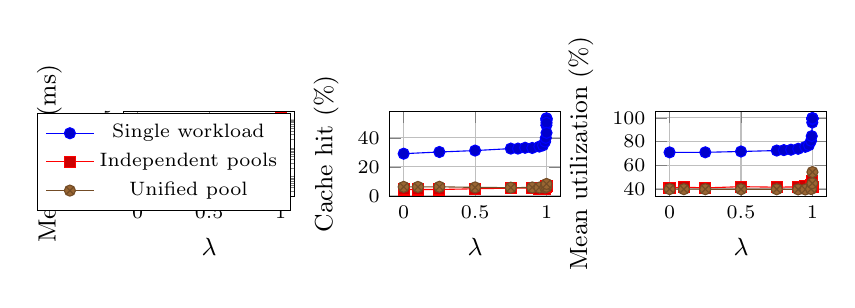
\begin{tikzpicture}
\begin{groupplot}[
group style={group size=3 by 1, horizontal sep=1.2cm},
width=0.31\textwidth, height=0.22\textwidth,
xlabel={$\lambda$}, grid=major, legend style={font=\scriptsize},
tick label style={font=\scriptsize}, label style={font=\small}]
\nextgroupplot[ylabel={Mean E2E (ms)},ymode=log]
\addplot coordinates {(0.00000,362.69544) (0.25000,362.69495) (0.50000,363.27757) (0.75000,364.33607) (0.80000,364.75942) (0.85000,365.84300) (0.90000,368.78518) (0.95000,379.10343) (0.97500,384.86009) (0.99000,399.08493) (0.99500,429.67505) (0.99900,724.85460) (0.99950,1174.74318) (0.99970,1708.78002) (0.99980,2443.54441) (0.99990,4461.56402) (0.99995,7791.37453) (1.00000,80115.35349)};
\addlegendentry{Single workload}
\addplot coordinates {(0.00000,376.62962) (0.10000,379.78270) (0.25000,378.68250) (0.50000,388.46968) (0.75000,395.56541) (0.90000,410.19108) (0.95000,426.15112) (0.99000,492.21342) (0.99900,1362.94680) (1.00000,114314.55595)};
\addlegendentry{Independent pools}
\addplot coordinates {(0.00000,347.84534) (0.10000,347.72060) (0.25000,347.59696) (0.50000,347.48507) (0.75000,347.44593) (0.90000,347.38493) (0.95000,347.77483) (0.99000,351.36325) (0.99900,374.77939) (1.00000,1746.14109)};
\addlegendentry{Unified pool}
\nextgroupplot[ylabel={Cache hit (\%)}]
\addplot coordinates {(0.00000,29.10617) (0.25000,30.27649) (0.50000,31.24932) (0.75000,32.61465) (0.80000,32.61978) (0.85000,33.18032) (0.90000,33.04614) (0.95000,33.99808) (0.97500,34.83316) (0.99000,37.43302) (0.99500,40.00057) (0.99900,48.69521) (0.99950,52.03669) (0.99970,53.18210) (0.99980,53.52253) (0.99990,52.95952) (0.99995,50.38813) (1.00000,43.46677)};
\addplot coordinates {(0.00000,4.49268) (0.10000,4.44205) (0.25000,4.43794) (0.50000,4.92795) (0.75000,5.37294) (0.90000,5.32711) (0.95000,4.94158) (0.99000,4.92207) (0.99900,6.38494) (1.00000,6.73287)};
\addplot coordinates {(0.00000,6.25765) (0.10000,6.21662) (0.25000,6.30699) (0.50000,5.88657) (0.75000,5.71234) (0.90000,5.84774) (0.95000,5.77186) (0.99000,5.79894) (0.99900,6.30170) (1.00000,8.27058)};
\nextgroupplot[ylabel={Mean utilization (\%)}]
\addplot coordinates {(0.00000,70.90656) (0.25000,70.95069) (0.50000,71.64826) (0.75000,72.44976) (0.80000,72.81293) (0.85000,73.16688) (0.90000,73.91270) (0.95000,75.57315) (0.97500,76.93804) (0.99000,80.66963) (0.99500,84.63610) (0.99900,96.12763) (0.99950,98.92229) (0.99970,99.67082) (0.99980,99.73953) (0.99990,99.73959) (0.99995,99.74055) (1.00000,99.38887)};
\addplot coordinates {(0.00000,40.84171) (0.10000,41.51941) (0.25000,40.90699) (0.50000,41.91897) (0.75000,41.49313) (0.90000,41.77077) (0.95000,42.76354) (0.99000,43.53937) (0.99900,46.53515) (1.00000,41.44585)};
\addplot coordinates {(0.00000,39.86486) (0.10000,39.82775) (0.25000,39.77821) (0.50000,39.73789) (0.75000,39.75241) (0.90000,39.62179) (0.95000,39.53588) (0.99000,39.93612) (0.99900,44.76044) (1.00000,54.26829)};
\end{groupplot}
\end{tikzpicture}
\caption{The CostScheduler tradeoff across the sampled $\lambda$ range. Lower $\lambda$ emphasizes online latency; higher $\lambda$ emphasizes execution efficiency.}
\label{fig:lambda-sweep}
\end{figure*}


\clearpage
\section{Request-Level Objective}
\label{sec:request-latency-objective}

The latency term in Section~\ref{sec:algorithm} normalizes every assignment by
its prompt length. This section isolates that design choice at $\lambda=0$ and
evaluates an alternative that treats every request as one latency observation.
The comparison is important because the scheduler predicts one execution
latency for a physical batch, while users observe that latency once per
request.

Using the token-normalized mass $U_n$ and request-assignment mass $S_n$
defined with Equation~\ref{eq:objective}, define the compact batch-weight
function
\begin{equation}
h_\kappa(x)=
\begin{cases}
x, & \kappa=0,\\[0.2em]
\dfrac{\log(1+\kappa x)}{\log\kappa}, & \kappa>1.
\end{cases}
\label{eq:request-weight}
\end{equation}
The two objectives then differ only in the argument of $h_\kappa$:
\begin{align}
J_{\mathrm{tok}}(W)
  &=\frac{1}{|\mathcal R|}\sum_{n\in\mathcal N}
    \bigl(L_n(\mathbf w_n)+Q_n\bigr)h_\kappa(U_n),
    \label{eq:token-latency-objective}\\
J_{\mathrm{req}}(W)
  &=\frac{1}{|\mathcal R|}\sum_{n\in\mathcal N}
    \bigl(L_n(\mathbf w_n)+Q_n\bigr)h_\kappa(S_n).
    \label{eq:request-latency-objective}
\end{align}
Here $L_n(\mathbf w_n)$ is predicted physical-batch execution latency and
$Q_n$ is predicted queue delay. Equation~\ref{eq:token-latency-objective}
emphasizes latency per prompt token: a request contributes $1/T_i$ assignment
mass. Equation~\ref{eq:request-latency-objective} instead counts every request
once, so a batch of $S_n$ requests contributes its predicted latency $S_n$
times when $\kappa=0$.

\subsection{Why the concave form creates larger batches}

For $\kappa>1$, the marginal batch weight is
\begin{equation}
h_\kappa'(x)=\frac{\kappa}{(1+\kappa x)\log\kappa}.
\label{eq:request-weight-derivative}
\end{equation}
In the measured traffic, $T_i$ ranges from 67 to 1,637 tokens. A request
therefore adds only $0.0006$--$0.015$ to $U_n$, but adds one to $S_n$.
At $\kappa=512$, the request-level argument consequently enters the low-slope
part of Equation~\ref{eq:request-weight-derivative} much sooner. Adding a
request to an existing batch then costs less objective mass than opening a new
batch on an empty node. This is the direct concentration pressure behind the
larger request-level batches. Token normalization is not a harmless global
rescaling here: it changes each request by a different $1/T_i$ factor and,
because $h_\kappa$ is nonlinear, also changes the curvature region traversed
by the optimizer.

\subsection{Why batching also increases without concavity}

The linear case, $\kappa=0$, has no saturation effect. Its request-level term
is the predicted sum of request latencies,
\begin{equation}
J_{\mathrm{req}}(W)=\frac{1}{|\mathcal R|}
\sum_{n\in\mathcal N}S_n\bigl(L_n(\mathbf w_n)+Q_n\bigr).
\label{eq:linear-request-latency-objective}
\end{equation}
Suppose another request is either packed onto node $n$ or starts a separate
batch on idle node $m$. The two incremental costs are
\begin{equation}
\begin{aligned}
\Delta_{\mathrm{pack}}
  &=(S_n+1)(L_n^{+}+Q_n)-S_n(L_n+Q_n),\\
\Delta_{\mathrm{open}}
  &=L_m^{(i)}+Q_m.
\end{aligned}
\label{eq:linear-pack-condition}
\end{equation}
The fitted Prefill latency surface grows sublinearly over part of the measured
batch range because fixed work is shared and the GPU processes requests
together. Where $\Delta_{\mathrm{pack}}<\Delta_{\mathrm{open}}$, the linear
objective therefore also selects a larger physical batch. In contrast, token
normalization makes a long request add little assignment mass while its work
can still increase $L_n$ for short requests already on that node. This
length-dependent cross-effect can favor separating requests even without a
concave weight. Removing $1/T_i$ aligns the objective with request-level
latency and removes that asymmetry.

This argument is conditional on the fitted latency surface, queue state, cache
state, and available nodes; it is not a claim that request-level weighting
must always create larger batches. Concavity adds an explicit concentration
force, while the linear result is an empirical property of the measured
Prefill regime.

\subsection{Real eight-GPU comparison}

We evaluate the two request-level variants on eight independent TP1 NVIDIA
H20 instances serving Qwen3.5-35B-A3B-FP8 in Prefill-only mode. Every run
uses the same 1,488-request stream, a 50-ms or 30-request collection window,
and 1,024-token cache blocks. We discard the first 744 requests and report the
last 744. The pre-fitted latency parameters initialize each Agent, but online
updates remain enabled. Schedule replay is disabled on the measured request
path. Prefill card-time is the sum of actual physical-batch execution time
across all eight GPUs; it measures occupied Prefill capacity rather than
instantaneous hardware utilization.

\begin{table}[t]
\centering
\small
\caption{Repeated real eight-GPU request-level objective results. Values are
means across the listed runs; brackets give the observed card-time range.
Card-time change is relative to the repeated FlexLB mean. Lower is better for
latency and card-time.}
\label{tab:request-latency-objective}
\textbf{(a) End-to-end latency}\\[0.35em]
\begin{tabular}{lrrrr}
\toprule
Policy / objective & Runs & Mean (ms) & P95 (ms) & Max (ms) \\
\midrule
FlexLB & 2 & 340.49 & 626.16 & 721.50 \\
Token-normalized, $\lambda=0$, $\kappa=512$
  & 2 & 317.30 & 593.66 & 652.72 \\
Token-normalized, $\lambda=0.5$, $\kappa=512$
  & 2 & \textbf{315.00} & 604.60 & 659.50 \\
Request-level, concave, $\kappa=512$
  & 3 & 318.71 & \textbf{595.85} & 712.82 \\
Request-level, linear, $\kappa=0$
  & 2 & 324.78 & 612.81 & 683.91 \\
\bottomrule
\end{tabular}

\vspace{0.8em}
\textbf{(b) Batching, occupied Prefill capacity, and prediction error}\\[0.35em]
\resizebox{\textwidth}{!}{%
\begin{tabular}{lrrrrr}
\toprule
Policy / objective & Runs & Mean batch & Card-time mean [range] (s) & vs. FlexLB & Master MAPE \\
\midrule
FlexLB & 2 & 2.30 & 32.48 [32.42, 32.54] & baseline & -- \\
Token-normalized, $\lambda=0$, $\kappa=512$
  & 2 & 3.24 & 24.40 [24.28, 24.52] & $-24.9\%$ & 6.14\% \\
Token-normalized, $\lambda=0.5$, $\kappa=512$
  & 2 & 3.18 & 24.41 [24.34, 24.48] & $-24.8\%$ & 7.04\% \\
Request-level, concave, $\kappa=512$
  & 3 & 4.20 & 21.02 [15.53, 24.21] & $-35.3\%$ & 7.09\% \\
Request-level, linear, $\kappa=0$
  & 2 & 4.23 & 20.56 [16.72, 24.40] & $-36.7\%$ & 6.85\% \\
\bottomrule
\end{tabular}
}
\end{table}

All four Cost variants reduce mean latency, P95, and occupied Prefill
card-time relative to the repeated FlexLB mean. The two token-normalized
variants are stable: both use approximately 24.4 card-s in each run. Their
mean-latency difference is only 0.7\%, while $\lambda=0$ has the better P95;
the repeated evidence therefore does not establish that $\lambda=0.5$ is
uniformly superior.

The request-level objectives show a different reliability profile. Concave
request weighting uses 15.53, 23.33, and 24.21 card-s across three runs;
linear weighting uses 16.72 and 24.40 card-s. Thus the previously observed
52.3\% reduction against FlexLB is a real high-batching outcome, but it is not
a representative steady-state result. The repeated means still reduce
card-time by 35.3\% and 36.7\%, although these means are pulled down by one
high-batching run per objective. Their typical non-outlier reductions are
approximately 25--28\%. Master total-latency MAPE remains between 6.1\% and
7.1\% after averaging, and every repeated run has zero unmatched physical
Batches. The variability therefore reflects objective and online scheduling
dynamics rather than failed request-to-Batch accounting.

\subsection{VLLM adapter validation with chunked Prefill}

We additionally validate the adapter on eight independent TP1 H20 VLLM
instances serving Qwen3.5-35B-A3B-FP8. Prefix caching and chunked Prefill are
enabled, generation is limited to one token, and the effective cache block
size is 1,056 tokens after VLLM's Mamba alignment. The Scheduler collects for
20 ms or 32 requests, with a maximum Master Batch size of 32. A Master Batch
may require several VLLM chunk iterations, but the adapter does not admit a
later Master Batch until every request in the active Batch has completed
Prefill. It reports that Batch exactly once. This preserves the scheduling
decision while allowing prompts up to 32k tokens to fit the engine budget.

Both policies receive the same 1,110-request, 7.31-million-token stream, start
with cold prefix caches, and use the same pre-fitted nine-parameter latency
state. Online fitting remains enabled. The traffic specification, adapter,
and initial state are verified by SHA-256 fingerprints before accepting a
run. All 1,110 requests return HTTP 200; prompt-token count, completion-token
count, finish reason, and a nonempty first token are checked for every
response. The FlexLB row uses our separately replicated Prefill selector,
not FlexLB's production Decode path.

\begin{table*}[t]
\centering
\small
\caption{Audited VLLM eight-GPU comparison. Mean Batch is the completed
NaviSched Master-Batch size, not a single VLLM forward width. Card-time sums
the interval from the first forward to final chunk completion on each GPU.
Changes are Cost relative to the FlexLB Prefill replica.}
\label{tab:vllm-real-comparison}
\resizebox{\textwidth}{!}{%
\begin{tabular}{lrrrrrrrrr}
\toprule
Policy & Mean & P50 & P95 & P99 & Mean Batch & Card-time & Cache hit & Node CV & Elapsed \\
 & \multicolumn{4}{c}{HTTP latency (ms)} & & (s) & (\%) & & (s) \\
\midrule
FlexLB Prefill replica
  & 3378.50 & 2858.20 & 8998.67 & 12883.46 & 1.087 & 290.732 & 24.24 & 0.1187 & 42.78 \\
Cost, $\lambda=0$
  & \textbf{2957.03} & \textbf{2821.52} & \textbf{4504.62} & \textbf{5103.52}
  & \textbf{1.572} & \textbf{282.469} & 19.21 & \textbf{0.0164} & \textbf{37.33} \\
Cost change
  & $-12.48\%$ & $-1.28\%$ & $-49.94\%$ & $-60.39\%$
  & $+44.62\%$ & $-2.84\%$ & $-5.03$ pp & $-86.2\%$ & $-12.73\%$ \\
\bottomrule
\end{tabular}%
}

\vspace{0.7em}
\resizebox{\textwidth}{!}{%
\begin{tabular}{llrrrrr}
\toprule
Policy & Prediction point & Predicted (ms) & Actual (ms) & Actual $-$ predicted (ms) & MAE (ms) & MAPE \\
\midrule
Cost & Master execution & 398.44 & 400.10 & +1.66 & 23.12 & 13.87\% \\
Cost & Agent pre-update execution & 398.73 & 400.10 & +1.37 & 16.54 & 11.45\% \\
Cost & Master total & 2884.51 & 2943.70 & +59.19 & 119.00 & 4.35\% \\
FlexLB replica & Master execution & 283.71 & 284.75 & +1.04 & 13.50 & 10.76\% \\
FlexLB replica & Agent pre-update execution & 283.52 & 284.75 & +1.23 & 11.58 & 9.87\% \\
FlexLB replica & Master total & 3310.26 & 3348.32 & +38.06 & 74.22 & 3.84\% \\
\bottomrule
\end{tabular}%
}
\end{table*}

Table~\ref{tab:vllm-real-comparison} shows that Cost reduces mean latency by
12.48\%, P95 by 49.94\%, and occupied Prefill card-time by 2.84\% in this
workload. Its larger Master Batches and much lower node card-time CV explain
the tail improvement. This is not a uniform improvement: P50 changes by only
1.28\%, and Cost obtains a lower Cache-hit rate than the FlexLB replica.

The 44.62\% increase in mean Master-Batch size does not imply a comparable
card-time reduction under chunked Prefill. Cost reduces the number of completed
Master Batches from 1,021 to 706, but their mean measured duration rises from
284.75 to 400.10 ms, or 40.51\%. Moreover, 355 of 706 Cost Master Batches
(50.3\%) require multiple VLLM chunk iterations, compared with 385 of 1,021
(37.7\%) for the FlexLB replica. Cost's lower Cache-hit rate also increases
executed miss tokens by 6.64\%, from 5.53M to 5.90M. After normalization by
miss tokens, Cost uses 47.86 versus 52.53 microseconds of card-time per token,
an 8.89\% efficiency improvement. Thus batching is beneficial, but the extra
miss work and multi-chunk composition offset most of its aggregate card-time
gain. The reported card-time also includes the short scheduling gaps between
chunk forwards; it is not pure GPU-kernel time.

The two chunking causes must be distinguished. The 131,072-token VLLM budget
limits aggregate tokens in one iteration and can be increased. Independently,
Qwen3.5 uses Mamba cache \texttt{align} mode when Prefix caching is enabled.
VLLM then forces Prefill to stop at the last complete 1,056-token effective
cache block before executing the remainder; for example, a 32,700-token prompt
is issued as 31,680 plus 1,020 tokens. Increasing the aggregate token budget
does not remove this alignment tail. Removing it requires disabling Prefix
caching, using block-aligned prompt lengths, or changing VLLM's Mamba cache
semantics; none is equivalent to the measured configuration.

We also replay the exact traffic through the simulator without time
compression. Cost produces 551 Master rounds and 685 completed Master Batches, versus
554 and 706 in the real run; its mean Batch size is 1.620 versus 1.572,
card-time is 279.554 versus 282.469 s, and Cache hit is 19.60\% versus 19.21\%.
Simulated execution is 408.11 ms, close to the real 400.10 ms. However,
simulated Queue time is 1998.28 ms versus 2543.60 ms in the real run. The
traffic sidecar records HTTP send time, but not each request's post-JSON,
post-Python arrival time at the Master; that missing timing changes burst
shape. We therefore use simulation to validate Batch accounting, card-time,
Cache, and execution trends, but do not claim that it reproduces absolute
end-to-end latency.

\subsection{Mean-weight-matched normalization power}

Changing the exponent in $1/T_i^p$ also changes the magnitude of the latency
term. To isolate the exponent, we choose a scale $c_p$ so that the mean
request weight $c_p/T_i^p$ under the measured token distribution matches the
$p=1$ mean. We retain $\lambda=0$, $\kappa=512$, and
$\alpha=4.8520302639$. Table~\ref{tab:normalization-power} reports the real
eight-GPU results.

\begin{table}[t]
\centering
\small
\caption{Mean-weight-matched normalization-power scan. Two-run rows report
the repeated mean; one-run rows remain exploratory. Changes are relative to
the repeated FlexLB mean.}
\label{tab:normalization-power}
\begin{tabular}{rrrrrrrr}
\toprule
$p$ & $c_p$ & Runs & Mean (ms) & P95 (ms) & Card-time (s) & Mean batch & MAPE \\
\midrule
1.00 & 1.000000 & 2 & 317.30 & 593.66 & 24.40 & 3.24 & 6.14\% \\
0.75 & 0.239890 & 1 & 318.67 & 611.76 & 24.35 & 3.17 & 5.90\% \\
0.50 & 0.056331 & 2 & \textbf{309.20} & \textbf{593.89} & 24.47 & 3.18 & 6.42\% \\
0.25 & 0.012911 & 2 & 319.32 & 610.70 & \textbf{23.35} & \textbf{3.35} & 6.52\% \\
0.00 & 0.002882 & 1 & 321.33 & 607.00 & 24.30 & 3.25 & 6.32\% \\
\bottomrule
\end{tabular}
\end{table}

The scan exposes a Pareto tradeoff rather than one universally best exponent.
$p=0.5$ gives the lowest repeated mean latency, 9.2\% below FlexLB and 2.6\%
below $p=1$, while preserving nearly the same P95 and card-time as $p=1$.
$p=0.25$ gives the lowest repeated card-time, 28.1\% below FlexLB, and the
largest mean Batch among the matched rows, but its mean latency is 3.3\%
higher than $p=0.5$. The $p=0$ and $p=0.75$ rows have only one run and are not
used to claim an optimum. These results cover one host, model, and request
stream; they do not establish a universal exponent across models or GPU types.

\FloatBarrier
\clearpage
\section{Decision-Snapshot Case Study}
\label{sec:decision-snapshot-case-study}

Aggregate metrics do not reveal why one scheduling decision was made. This
section therefore reconstructs one snapshot sampled from the real eight-GPU
run, evaluates all $8^2=64$ discrete assignments, and traces the projected
gradient iterations that produced the returned route. Request features, node
state, fitted latency parameters, and optimizer initialization are fixed
throughout. The alternative assignments are counterfactual predictions, not
model-server executions; their values must not be read as measured
end-to-end latency.

\subsection{Captured decision state}

The window contains two requests, $r_0$ and $r_1$, with 820 and 220 prompt
tokens. They have already waited 31 and 8 ms for the collection window. Both
requests are cache misses on all eight nodes, so Cache cannot distinguish the
candidates. Table~\ref{tab:decision-node-state} gives the remaining state.
$L_{820}$ and $L_{220}$ are predicted execution times when each request runs
alone; $L_{820+220}$ is the prediction when both form one physical batch.

The surrounding Replay-enabled real run sampled 29 distinct Master scheduling
rounds containing 50 requests: 8 rounds contained one request and 21 contained
two, for a mean of 1.724 requests per round. The highlighted case therefore
uses the sample maximum of \keydata{two requests}. This distribution is a
diagnostic sample, not a statistic from the final 1,488-request performance
run: that run deliberately disabled Replay and did not persist per-request
schedule IDs. Reporting the sampled distribution as the final steady-state
distribution would therefore be invalid. The current Master now accumulates
schedule-round count, total requests, minimum, maximum, mean, and a
requests-per-round histogram directly in its snapshot. This requires no
Replay and stores no request payload; it makes the distribution available to
future real runs but cannot retroactively reconstruct the historical run.

\begin{table}[t]
\centering
\small
\caption{Node state and fitted Prefill predictions at the captured decision.
All times are milliseconds. The one-batch prediction is lower than either
single-request prediction because the fitted surface captures shared GPU
work within a physical batch.}
\label{tab:decision-node-state}
\begin{tabular}{rrrrrr}
\toprule
Node & Inflight & Predicted queue & $L_{820}$ & $L_{220}$ & $L_{820+220}$ \\
\midrule
0 & 0 & 0.000 & 187.225 & 245.797 & 171.495 \\
1 & 1 & 40.735 & 197.230 & 255.777 & 181.429 \\
2 & 0 & 0.000 & 187.087 & 245.604 & \keydata{171.366} \\
3 & 1 & 29.347 & 194.695 & 253.272 & 178.915 \\
4 & \alertdata{0} & \alertdata{109.923} & 198.935 & 257.493 & 183.126 \\
5 & 0 & 0.000 & 187.741 & 246.307 & 172.013 \\
6 & 0 & 0.000 & 194.829 & 253.382 & 179.047 \\
7 & 0 & 0.000 & 194.225 & 252.790 & 178.443 \\
\bottomrule
\end{tabular}
\end{table}

Nodes 1, 3, and 4 carry 40.735, 29.347, and 109.923 ms of predicted queue
delay. The highlighted node-4 values are not contradictory: inflight is the
latest Agent-reported number of accepted requests, whereas the Queue used by
the scheduler is an effective availability estimate. After a scheduling
decision, the Master immediately adds a pending Batch reservation to that
estimate so that another scheduling round cannot treat the target as idle
while the request is in transit. The Agent may therefore still report zero
inflight while the Master correctly reserves positive future GPU time. The
Replay records the resulting effective Queue but does not serialize the base
Agent Queue and reservation components separately; 109.923 ms is known to
have affected this decision, but its acknowledgment phase cannot be recovered
from this JSON alone. Among the queue-free nodes, node 2 has the lowest
predicted one-batch time. Separating the requests is intrinsically expensive:
even the best queue-free split, $(0,2)$, consumes 432.829 ms of predicted
card-time, compared with 171.366 ms for batching both requests on node 2.

\subsection{One decision under representative objectives}

Let a node pair $(n_0,n_1)$ denote the destinations of $r_0$ and $r_1$.
Every comparison uses $\lambda=0$, $\kappa=128$, and 50 iterations unless the
row is explicitly linear. Therefore the raw execution term is diagnostic and
has zero weighted contribution; the selected objective is one half of the raw
latency term. Table~\ref{tab:decision-snapshot} compares the returned route
with the exact discrete minimum obtained by enumerating all 64 pairs.

\begin{table}[t]
\centering
\small
\caption{Decision quality on one real eight-GPU snapshot. ``Best'' is the
minimum among all 64 node pairs; ``selected'' is the route returned by
projected gradient descent. The Cost gap is relative to the discrete minimum
under the same objective.}
\label{tab:decision-snapshot}
\begin{tabular}{llrrrr}
\toprule
Objective & Case & Route & Rank & Cost & Cost gap \\
\midrule
Token normalized & Best & \keydata{$(2,2)$} & 1 & \keydata{9.760} & 0.00\% \\
Token normalized & Selected & $(5,5)$ & 3 & 9.797 & +0.38\% \\
Request concave & Best & \keydata{$(2,2)$} & 1 & \keydata{97.992} & 0.00\% \\
Request concave & Selected & $(7,7)$ & 4 & 102.039 & +4.13\% \\
Matched $p=0.25$ & Best & \keydata{$(2,2)$} & 1 & \keydata{9.760} & 0.00\% \\
Matched $p=0.25$ & Selected & \alertdata{$(7,5)$} & \alertdata{18} & \alertdata{14.449} & \alertdata{+48.04\%} \\
Request linear & Best & \keydata{$(2,2)$} & 1 & \keydata{171.366} & 0.00\% \\
Request linear & Selected & $(5,5)$ & 3 & 172.013 & +0.38\% \\
\bottomrule
\end{tabular}
\end{table}

\begin{table}[t]
\centering
\small
\caption{Predicted Cost decomposition for the same best and returned routes.
The execution and latency columns are the unweighted raw terms; card-time and
request mean are counterfactual model predictions, not measured executions.}
\label{tab:decision-snapshot-components}
\begin{tabular}{llrrrrr}
\toprule
Objective & Case & Exec. raw & Lat. raw & Cost & Card-time & Req. mean \\
\midrule
Token normalized & Best & 342.732 & 19.520 & 9.760 & 171.366 & 171.366 \\
Token normalized & Selected & 344.026 & 19.594 & 9.797 & 172.013 & 172.013 \\
Request concave & Best & 342.732 & 195.984 & 97.992 & 171.366 & 171.366 \\
Request concave & Selected & 356.886 & 204.078 & 102.039 & 178.443 & 178.443 \\
Matched $p=0.25$ & Best & 342.732 & 19.520 & 9.760 & 171.366 & 171.366 \\
Matched $p=0.25$ & Selected & 440.532 & 28.898 & 14.449 & 440.532 & 220.266 \\
Request linear & Best & 342.732 & 342.732 & 171.366 & 171.366 & 171.366 \\
Request linear & Selected & 344.026 & 344.026 & 172.013 & 172.013 & 172.013 \\
\bottomrule
\end{tabular}
\end{table}

\subsection{Cross-objective and per-Batch accounting}

Absolute Cost values cannot be compared across normalization schemes because
their weight scales differ. Ranks can be compared: each fixes one returned
route and evaluates it against all 64 candidates under the indicated column's
objective. Table~\ref{tab:decision-cross-cost} separates the quality of a
route from the optimizer that happened to return it.

\begin{table}[t]
\centering
\small
\caption{Cross-evaluation of every returned route. Each Cost/rank cell is
recomputed under the column objective. Green marks the efficient co-located
route shared by two optimizers; red marks the split route that is poor under
all four objectives, rather than merely under the objective that produced it.}
\label{tab:decision-cross-cost}
\begin{tabular}{llrrrrr}
\toprule
Returned by & Route & Token norm. & Request concave & Matched $p=.25$ & Request linear & Card-time \\
\midrule
Token normalized & \keydata{$(5,5)$} & 9.7969 / 3 & 98.3623 / 3 & 9.7969 / 3 & 172.0131 / 3 & 172.013 \\
Request concave & $(7,7)$ & 10.1631 / 4 & 102.0392 / 4 & 10.1631 / 4 & 178.4431 / 4 & 178.443 \\
Matched $p=.25$ & \alertdata{$(7,5)$} & \alertdata{14.5426 / 18} & \alertdata{220.6194 / 22} & \alertdata{14.4489 / 18} & \alertdata{220.2661 / 20} & \alertdata{440.532} \\
Request linear & \keydata{$(5,5)$} & 9.7969 / 3 & 98.3623 / 3 & 9.7969 / 3 & 172.0131 / 3 & 172.013 \\
\bottomrule
\end{tabular}
\end{table}

The matched route is therefore not a specialization that scores well only
under its own normalization. It ranks 18th, 22nd, 18th, and 20th under the
four objectives. Conversely, $(5,5)$ ranks third under every objective. This
is direct evidence that the abnormal split is an optimizer-path failure, not
a disagreement among the four discrete optima.

For complete arithmetic, let $U_n$ be the summed request-linear quantity for
the requests assigned to node $n$, $L_n$ the fitted Batch execution time,
$Q_n$ the effective Queue, and $z_n=\sum_{i\rightarrow n}w_i$ the assignment
mass. Because this snapshot has $\lambda=0$ and two requests, each Batch adds
$(L_n+Q_n)h(z_n)/2$ to total Cost. Table~\ref{tab:decision-batch-cost}
shows every Batch created by the four returned routes.

\begin{table}[t]
\centering
\footnotesize
\caption{Batch formation and fitted execution for every returned decision.
The two red rows are separate physical Batches created by matched $p=.25$.
Execution and Queue columns are milliseconds.}
\label{tab:decision-batch-cost}
\begin{tabular}{llrrr}
\toprule
Objective & Route/node/requests & $U_n$ & $L_n$ & $Q_n$ \\
\midrule
Token norm. & $(5,5)$/5/$r_0+r_1$ & 116.504522 & 172.013150 & 0 \\
Request concave & $(7,7)$/7/$r_0+r_1$ & 116.615013 & 178.443140 & 0 \\
Matched $p=.25$ & \alertdata{$(7,5)$/5/$r_1$} & 23.136403 & 246.307126 & 0 \\
Matched $p=.25$ & \alertdata{$(7,5)$/7/$r_0$} & 93.438078 & 194.225011 & 0 \\
Request linear & $(5,5)$/5/$r_0+r_1$ & 116.504522 & 172.013150 & 0 \\
\bottomrule
\end{tabular}
\end{table}

\begin{table}[t]
\centering
\footnotesize
\caption{Nonlinear weighting and final Cost contribution for the same
Batches. The matched contributions in red sum to 14.448895.}
\label{tab:decision-batch-weight}
\begin{tabular}{llrrrr}
\toprule
Objective & Route/node & $z_n$ & $h(z_n)$ & $(L_n+Q_n)h(z_n)$ & Cost contribution \\
\midrule
Token norm. & $(5,5)$/5 & 0.005764967 & 0.113908306 & 19.593726 & 9.796863 \\
Request concave & $(7,7)$/7 & 2.000000000 & 1.143660650 & 204.078398 & 102.039199 \\
Matched $p=.25$ & \alertdata{$(7,5)$/5} & 0.003352307 & 0.073586023 & 18.124762 & \alertdata{9.062381} \\
Matched $p=.25$ & \alertdata{$(7,5)$/7} & 0.002412659 & 0.055466736 & 10.773027 & \alertdata{5.386514} \\
Request linear & $(5,5)$/5 & 2.000000000 & 2.000000000 & 344.026300 & 172.013150 \\
\bottomrule
\end{tabular}
\end{table}

The matched split loses the physical-Batch saving before weighting is even
applied: it predicts 246.307 ms for $r_1$ on node 5 and 194.225 ms for $r_0$
on node 7, totaling 440.532 card-ms. Co-locating both on node 2 predicts
171.366 card-ms. The two nonlinear contributions, 18.124762 and 10.773027,
then produce $(18.124762+10.773027)/2=14.448895$.

\subsection{Cost reconstruction}

For the token-normalized selected route, both requests go to node 5. Their
assignment mass is $1/820+1/220=0.005765$, giving
$h_{128}(0.005765)=0.113908$. With $L_5=172.013$ ms and $Q_5=0$,
\begin{equation}
J_{\mathrm{tok}}(5,5)
=\frac{172.013\times0.113908}{2}=9.7969.
\end{equation}
The exact best route, $(2,2)$, has the same one-batch structure but a slightly
lower fitted execution time, producing Cost 9.760. The returned route is only
0.38\% above the discrete minimum.

For request-level concave weighting, $(7,7)$ has assignment mass two and
$h_{128}(2)=1.143661$. Its Cost is
$178.443\times1.143661/2=102.039$, 4.13\% above the discrete minimum on node 2.
The matched $p=0.25$ route is qualitatively different. The long request goes
to node 7 and contributes
$194.225\times h_{128}(0.002413)=10.773$; the short request goes to node 5 and
contributes $246.307\times h_{128}(0.003352)=18.125$. Their sum divided by two
is 14.449. This split is ranked 18th and consumes 157.1\% more predicted
card-time than $(2,2)$. Finally, linear request-level weighting gives
$h_0(2)=2$, so $(5,5)$ has Cost $172.013\times2/2=172.013$ and is again only
0.38\% above the discrete minimum.

\subsection{Optimization path and explanation}

All four runs start from the same random relaxed assignment, whose largest
weights point to nodes $(4,6)$. Table~\ref{tab:decision-optimization-path}
shows what projection does next. ``Alternates'' means successive projected
solutions switch between the two listed pairs; the loss is evaluated before
the following update, and the lower evaluated pair is retained.

\begin{table}[t]
\centering
\small
\caption{Projected optimization path for the captured decision.}
\label{tab:decision-optimization-path}
\begin{tabular}{lrrr}
\toprule
Objective & First projection & Later behavior & Returned \\
\midrule
Token normalized & $(7,5)$ & settles at $(5,5)$ & $(5,5)$ \\
Request concave & $(7,7)$ & remains $(7,7)$ & $(7,7)$ \\
Matched $p=0.25$ & $(7,5)$ & alternates $(7,5)/(5,7)$ & $(7,5)$ \\
Request linear & $(5,5)$ & remains $(5,5)$ & $(5,5)$ \\
\bottomrule
\end{tabular}
\end{table}

The normalization change therefore affects more than the mathematical ranking
of already-discrete routes. With fixed $\alpha=128$, it rescales the gradient;
the first projected step is nearly one-hot and places the optimizer in a
different basin. The matched $p=0.25$ run then oscillates between two split
assignments and never reaches the much better co-located candidates. This
explains the otherwise surprising non-monotonic Batch and card-time changes:
they are an interaction among objective scale, fixed step size, simplex
projection, and the non-convex fitted latency surface. They are not evidence
that request-level weighting intrinsically prefers the returned nodes.

The scene also bounds what can be inferred. It exposes a concrete relaxation
and optimization-quality gap, but it does not predict the end-to-end result of
a different policy because that policy changes subsequent queues and online
model updates. Consequently Table~\ref{tab:request-latency-objective} remains
the performance evidence, while this section explains one decision and
identifies step-size normalization as a separate algorithmic issue.

\subsection{Discrete-selection repair and regression gate}
\label{sec:discrete-repair}

The deployed route is discrete even though the optimizer state is continuous.
Retaining only the lowest continuous objective is therefore insufficient: an
apparently better fractional solution can collapse under per-request
$\arg\max$ selection. We evaluate the actual discrete objective every five
iterations. If its relative gap from the continuous objective exceeds 25\%,
the remaining iterations reduce the step size by a factor of 0.7 and evaluate
the discrete route after every update. The scheduler retains the lowest
discrete objective observed under the original loop and time budgets. The
check aggregates selected requests by node in $O(|\mathcal R|+|\mathcal N|)$
time; it neither constructs a request--node one-hot matrix nor uses
categorical sampling.

Table~\ref{tab:discrete-collapse-repair} gives the failure that triggered this
change. The continuous objective falls from 88.009 to 83.753, but that number
is not used to compare the returned routes. Before the repair, all 12 requests
select node 13 and the resulting discrete objective is 547.887. The repair
detects a 451.9\% gap at iteration 5 and retains the best discrete route found
at iteration 19. That route uses nodes
$[7,24,19,1,31,1,11,6,11,28,27,28]$, forms nine batches, and reduces the
discrete objective to 97.618. Later iterations may still lower the continuous
objective, but they cannot overwrite this better discrete result.

\begin{table}[t]
\centering
\caption{Repair of the captured 12-request, 32-node collapse. Continuous
loss describes the relaxed state; the discrete objective evaluates the route
that is actually returned.}
\label{tab:discrete-collapse-repair}
\small
\begin{tabular}{lrrrr}
\toprule
Version & Continuous loss & Discrete objective & Nodes used & Batches \\
\midrule
Before repair & 88.009 & \alertdata{547.887} & 1 & 1 \\
Discrete repair & 83.753 & \keydata{97.618} & 9 & 9 \\
\bottomrule
\end{tabular}
\end{table}

A fix to route selection is acceptable only if it also preserves a previously
valid workload. Table~\ref{tab:discrete-repair-regression} applies this gate.
The v19 workload uses the same 1,488 requests, eight nodes, 50-ms collection
window, $\lambda=0$, request-level latency, concavity 512, and step size
4.852. Its two repaired runs reduce prefill card-time by 4.32\% and 6.45\%
relative to the original run, so the earlier card-time benefit does not
regress. This does not imply that every metric improves: mean latency rises in
both v19 repetitions. Medium requests improve in both card-time and latency.
For long requests, two repetitions are stable while one valid repetition has
more physical co-batching and substantially higher mean latency; we retain
that outlier rather than selecting only favorable runs.

\begin{table}[t]
\centering
\caption{Simulation regression after discrete selection repair. Values are
means over the stated stable runs; card-time change is relative to the
corresponding pre-repair runs. Lower card-time and latency are better.}
\label{tab:discrete-repair-regression}
\small
\begin{tabular}{lrrrrr}
\toprule
Workload & Runs & Batch before/after & Card-time before/after (s) & Change & Mean latency before/after (ms) \\
\midrule
v19 short & 1/2 & 5.952 / 6.615 & 14.849 / 14.049 & \keydata{-5.39\%} & 212.35 / \alertdata{231.16} \\
4k/8k & 2/2 & 6.465 / 2.273 & 4540.42 / 4053.10 & \keydata{-10.73\%} & 14931.38 / \keydata{4910.40} \\
16k/32k & 2/2 & 1.190 / 1.141 & 22651.70 / 22644.14 & -0.03\% & 37540.46 / \keydata{35444.47} \\
\bottomrule
\end{tabular}
\end{table}

\FloatBarrier
\subsection{Production-range length regression}

We next extend the repaired scheduler over the serving prompt range rather
than extrapolating from the v19 short-request trace. The mixed workload sends
1,600 requests spanning 128, 256, 512, 1k, 2k, 4k, 8k, 16k, 32k, and 64k
tokens to 64 simulated Agents. Requests retain their recorded arrival times;
the Master uses a 50-ms collection window and the simulator runs without time
compression. We discard the first 20\% of each run. The two boundary
workloads separately exercise 4,000 prompts from 128--2k tokens and 160
isolated 64k prompts. All runs are cache misses so that this experiment
isolates batching and queue placement. The baseline is NaviSched's
maximum-cache-hit policy acting as a cache-only proxy; it is not a measurement
of the RTP-LLM FlexLB implementation.

Every row in Table~\ref{tab:production-range-repair} uses archive SHA prefix
\code{d2b289107f70}, the same fitted parameters, and two repetitions. The
runtime readback confirms $\lambda=0$, request-level linear latency,
$\alpha=4.85203$, one fit update per sample, and the 5/0.25/0.7 discrete
check, gap, and decay settings. All requests complete, no physical batch
exceeds 65,536 tokens, and the prediction column compares the value available
to the scheduling decision with the subsequently observed value.

\begin{table}[h]
\centering
\caption{No-compression simulation across the production prompt range after
the discrete-selection repair. Values are means of two audited repetitions;
card-time is the sum of simulated prefill execution over all Agents.}
\label{tab:production-range-repair}
\scriptsize
\begin{tabular}{llrrrrr}
\toprule
Workload & Policy & Batch & Card-time (s) & Mean (ms) & P95 (ms) & Pred. MAPE \\
\midrule
128--2k & Cache proxy & 1.151 & 334.62 & \keydata{145.85} & \keydata{228.70} & 0.124\% \\
128--2k & Cost & 2.108 & \keydata{233.57} & \alertdata{161.93} & \alertdata{264.24} & 0.184\% \\
128--64k mixed & Cache proxy & 1.061 & \keydata{7648.09} & \alertdata{45333.76} & \alertdata{199721.85} & 0.046\% \\
128--64k mixed & Cost & 1.752 & \alertdata{7658.53} & \keydata{4708.05} & \keydata{11173.47} & 0.042\% \\
Isolated 64k & Cache proxy & 1.000 & 28792.28 & \alertdata{273969.17} & \alertdata{533251.40} & 0.002\% \\
Isolated 64k & Cost & 1.000 & 28792.28 & \keydata{180011.11} & \keydata{180012.25} & 0.000\% \\
\bottomrule
\end{tabular}
\end{table}

\FloatBarrier
The table reports the batch-efficiency, card-time, latency, and prediction
effects together so that a lower value in one column is not mistaken for a
universal improvement. For short prompts, Cost reduces card-time by 30.2\%
but raises mean latency by 11.0\%. In the mixed workload it reduces mean and
P95 latency by 89.6\% and 94.4\%, respectively, while card-time is 0.14\%
higher than the proxy. Isolated 64k requests cannot co-batch, so both policies
perform the same compute; Cost instead avoids node queue concentration and
reduces the mean and tail delay. These results establish internal simulator
consistency over the measured prompt range, not cross-model or cross-GPU
generalization.

The excluded long-run outlier is not a failed run: all 640 steady requests
complete and prediction MAPE is effectively zero. Its mean batch rises to
1.725, card-time rises by 0.78\%, and mean latency reaches 52.75 s. The Master
still schedules exactly two requests per round; the variation occurs when
adjacent decisions reach the same simulated Agent and become one physical
batch. This exposes event-order sensitivity in the long-request simulator and
prevents a claim that every configuration or every repetition improves.

\FloatBarrier
\section{Discussion}

\paragraph{Freshness versus overhead.}
Every completed batch can change queue and cache state. Reporting immediately
improves decisions but consumes control-plane capacity. \system currently
prioritizes ordered event fidelity; periodic coalescing and its effect on
route quality remain an explicit experiment rather than an assumed-safe
optimization.

\paragraph{Continuous versus discrete objectives.}
The concave weight can narrow a relaxation mismatch, but it does not make
projected gradient descent a proof of global optimality. The explicit
discrete check in Section~\ref{sec:discrete-repair} prevents a lower
continuous loss from overwriting a better returned route. It remains an
engineering safeguard rather than an exhaustive solver; alternative discrete
or sparse methods must be compared under the same decision-time budget.

\paragraph{Shared pools.}
Pooling creates more cache-placement and batching choices, but it also allows
long and short prompts to interact. A shared-pool result is useful only when
per-source latency is retained. This is why the simulator records each source
label for metrics even though the unified scheduler deliberately ignores that
label when making a route.

\section{Related Work}

Orca introduced iteration-level scheduling for transformer serving, while
vLLM's PagedAttention made KV memory allocation efficient and flexible
\cite{orca,vllm}. Sarathi-Serve studies chunked-prefill scheduling to control
latency interference~\cite{sarathi}. These systems primarily optimize work
inside a model-serving replica; \system consumes their real batch and cache
events to make a cluster-level prefill choice.

DistServe and Splitwise demonstrate the latency and goodput benefits of
separating prefill from decode~\cite{distserve,splitwise}. Mooncake further
centers disaggregated serving around KV-cache transfer and storage
\cite{mooncake}. \system is complementary: it provides a replaceable routing
and state plane for a prefill fleet, without defining the decode transport or
KV tensor movement protocol.

SGLang exposes prefix-aware execution through RadixAttention, and CacheBlend
studies reuse for retrieval-augmented prompts~\cite{sglang,cacheblend}. These
works reinforce that prefix state changes request cost. \system contributes a
distributed mirror, an online batch model, and a policy that balances that
state with queueing and batch composition.

\section{Limitations}

The evaluation combines a trace-driven logical executor with physical
eight-GPU RTP-LLM Prefill runs. Simulator utilization is logical executor busy
time and cannot capture kernel occupancy, memory stalls, or power; the
hardware tables therefore use observed Prefill card-time instead. Current
physical results cover one H20 host and one Qwen3.5 model, so they do not
establish transfer across GPU types or model families.

The current objective uses a dense request-node matrix and is not intended to
claim unbounded cluster scale. Cache hashes reveal equality patterns even
though they omit prompt text; deployments must protect the control plane
accordingly. Full cache synchronization briefly locks the Agent cache set, an
acceptable initial recovery path but a target for incremental snapshotting.
Finally, adapter correctness depends on reproducing the model runtime's exact
block hash and observing its true queue. A framework hook after internal
waiting omits that earlier wait from Agent queue state and must be documented
as an observability boundary.

The raw production-derived traffic logs may not be redistributable. The
repository retains the machine-readable aggregate report, objective-ablation
data, replay examples, generation scripts, and all simulator code, while a
full external rerun requires traces with the documented schema and timing.

\section{Conclusion}

Distributed prefill scheduling requires joint state and optimization; address
selection alone is insufficient. It links request
features, per-node cache state, actual batch execution, and online latency
models while preserving the model framework's native data path. Its scheduler
forms a constrained differentiable assignment, evaluates discrete routes in a
bounded repair phase, and runs optimization as alternating parallel dataflow
stages. The resulting system is extensible, replayable, and explicit about the
tradeoff among route quality, execution efficiency, and decision time.

\appendix
\section{Experimental Tables}

% Generated by generate_artifacts.py; do not edit.
\newcommand{\ExperimentGeneratedAt}{2026-08-24T03:13:55.088107+00:00}

\begin{table*}[t]
\centering
\scriptsize
\setlength{\tabcolsep}{2.4pt}
\caption{Single-workload strategy comparison. Utilization is logical busy time divided by logical elapsed time.}
\label{tab:strategy-baseline}
\begin{tabular}{lrrrrrrrrrrr}
\toprule
Scheduler & $\lambda$ & Loops & Req./sched. & Sched. ms & Queue & Exec. & E2E & P99 & Cache & Util. & QPS \\
\midrule
random & -- & -- & 6.5 & 0.014 & 75767.26 & 353.10 & 76140.78 & 148277.11 & 13.0 & 99.7 & 113.8 \\
max\_cache\_hit & -- & -- & 6.5 & 0.094 & 87278.33 & 360.32 & 87659.14 & 537843.90 & 43.7 & 99.8 & 56.3 \\
cost & 0.5 & 50.0 & 6.5 & 6.150 & 2.78 & 333.82 & 363.28 & 426.20 & 31.2 & 71.6 & 178.1 \\
\bottomrule
\end{tabular}
\par\vspace{3pt}
\begin{minipage}{0.98\textwidth}
\footnotesize The table compares scheduler overhead and service outcomes under the same single-workload trace to test whether joint cost-aware routing avoids overload. CostScheduler preserves the offered 178.1 QPS with low queueing, whereas random and cache-only routing build long queues despite lower overhead or higher cache hit rate.
\end{minipage}
\end{table*}

\begin{table*}[t]
\centering
\scriptsize
\setlength{\tabcolsep}{2.4pt}
\caption{Trace composition and per-source outcomes in the unified CostScheduler run at lambda zero.}
\label{tab:workloads}
\begin{tabular}{lrrrrrrrr}
\toprule
Trace & Requests & Share & Mean & P50 & P90 & P99 & Cache & Batch \\
\midrule
agent\_biz\_4091 & 51815 & 57.4 & 6465.0 & 2746 & 21270 & 30828 & 17.2 & 2.22 \\
agent\_biz\_69eb & 19819 & 22.0 & 65014.4 & 59188 & 103802 & 124609 & 7.1 & 1.02 \\
agent\_biz\_aae5 & 4504 & 5.0 & 92667.1 & 70789 & 150959 & 409817 & 6.2 & 1.02 \\
agent\_biz\_f233 & 10299 & 11.4 & 8277.0 & 4272 & 23576 & 30874 & 14.2 & 2.96 \\
agent\_biz\_ddec & 3854 & 4.3 & 234290.2 & 186141 & 395937 & 786440 & 0.3 & 1.01 \\
\bottomrule
\end{tabular}
\par\vspace{3pt}
\begin{minipage}{0.98\textwidth}
\footnotesize The table characterizes the five source traces mixed into one pool so aggregate results can be interpreted against workload skew. Mean prompt length spans 6.5k to 234k tokens, and the longest source has both the lowest cache hit rate and almost no batching.
\end{minipage}
\end{table*}

\begin{table*}[t]
\centering
\scriptsize
\setlength{\tabcolsep}{2.4pt}
\caption{Objective ablation on identical schedule contexts. All loop counts are measured rather than configured values.}
\label{tab:objective-ablation}
\begin{tabular}{llrrrrrrr}
\toprule
Weight & $\lambda$ & Loops & Queue & Exec. & E2E & P99 & Cache & Batch \\
\midrule
linear & 0.0 & 2 & 3.23 & 331.92 & 355.89 & 567.09 & 22.6 & 1.77 \\
linear & 0.0 & 50 & 24.14 & 325.35 & 376.55 & 619.55 & 16.8 & 1.50 \\
$\log(1+128x)/128$ & 0.0 & 2 & 0.86 & 329.90 & 351.53 & 462.31 & 27.0 & 2.43 \\
$\log(1+128x)/128$ & 0.0 & 5 & 0.35 & 327.60 & 349.01 & 421.02 & 25.5 & 2.32 \\
$\log(1+128x)/128$ & 0.0 & 10 & 0.26 & 327.20 & 349.28 & 415.67 & 24.7 & 2.29 \\
$\log(1+128x)/128$ & 0.0 & 20 & 0.16 & 326.77 & 350.08 & 401.25 & 24.3 & 2.27 \\
$\log(1+128x)/128$ & 0.0 & 50 & 0.25 & 326.59 & 353.83 & 398.65 & 22.8 & 2.22 \\
linear & 0.1 & 50 & 23.82 & 324.73 & 375.41 & 600.97 & 17.8 & 1.49 \\
$\log(1+128x)/128$ & 0.1 & 50 & 0.21 & 326.27 & 353.25 & 392.73 & 23.1 & 2.21 \\
linear & 0.5 & 50 & 60.21 & 323.96 & 411.11 & 711.75 & 19.6 & 1.48 \\
$\log(1+128x)/128$ & 0.5 & 50 & 0.97 & 325.88 & 353.79 & 409.52 & 23.5 & 2.13 \\
\bottomrule
\end{tabular}
\par\vspace{3pt}
\begin{minipage}{0.98\textwidth}
\footnotesize The table compares linear and logarithmic latency weights on identical scheduling contexts to test the dispersion correction. The logarithmic weight prevents queue growth at deeper optimization; five loops gives the lowest E2E at lambda zero, while further loops mainly improve the projected objective.
\end{minipage}
\end{table*}

\begin{table*}[t]
\centering
\scriptsize
\setlength{\tabcolsep}{2.4pt}
\caption{Single-workload CostScheduler sweep.}
\label{tab:single-lambda}
\begin{tabular}{lrrrrrrrrrrr}
\toprule
Run & $\lambda$ & Loops & Req./sched. & Sched. ms & Queue & Exec. & E2E & P99 & Cache & Util. & QPS \\
\midrule
l0 & 0.0 & 50.0 & 6.5 & 6.290 & 2.51 & 333.29 & 362.70 & 424.11 & 29.1 & 70.9 & 178.0 \\
l0\_25 & 0.25 & 50.0 & 6.5 & 6.162 & 2.53 & 333.48 & 362.69 & 424.33 & 30.3 & 71.0 & 178.1 \\
l0\_5 & 0.5 & 50.0 & 6.5 & 6.150 & 2.78 & 333.82 & 363.28 & 426.20 & 31.2 & 71.6 & 178.1 \\
l0\_75 & 0.75 & 50.0 & 6.5 & 6.361 & 3.17 & 334.21 & 364.34 & 427.79 & 32.6 & 72.4 & 178.1 \\
l0\_8 & 0.8 & 50.0 & 6.5 & 6.311 & 3.53 & 334.31 & 364.76 & 430.72 & 32.6 & 72.8 & 178.0 \\
l0\_85 & 0.85 & 50.0 & 6.5 & 6.344 & 4.41 & 334.43 & 365.84 & 439.29 & 33.2 & 73.2 & 178.1 \\
l0\_9 & 0.9 & 50.0 & 6.5 & 6.307 & 7.32 & 334.54 & 368.79 & 487.39 & 33.0 & 73.9 & 178.1 \\
l0\_95 & 0.95 & 50.0 & 6.5 & 6.453 & 16.82 & 335.19 & 379.10 & 731.98 & 34.0 & 75.6 & 178.1 \\
l0\_975 & 0.975 & 50.0 & 6.5 & 6.362 & 21.89 & 335.97 & 384.86 & 832.95 & 34.8 & 76.9 & 178.0 \\
l0\_99 & 0.99 & 50.0 & 6.5 & 6.271 & 33.88 & 338.28 & 399.08 & 933.97 & 37.4 & 80.7 & 177.9 \\
l0\_995 & 0.995 & 50.0 & 6.5 & 6.375 & 61.97 & 340.68 & 429.68 & 1107.03 & 40.0 & 84.6 & 178.1 \\
l0\_999 & 0.999 & 50.0 & 6.5 & 6.309 & 350.59 & 347.37 & 724.85 & 2018.26 & 48.7 & 96.1 & 178.1 \\
l0\_9995 & 0.9995 & 50.0 & 6.5 & 6.347 & 798.58 & 349.20 & 1174.74 & 3093.01 & 52.0 & 98.9 & 177.8 \\
l0\_9997 & 0.9997 & 50.0 & 6.5 & 6.419 & 1331.98 & 349.75 & 1708.78 & 4250.17 & 53.2 & 99.7 & 177.8 \\
l0\_9998 & 0.9998 & 50.0 & 6.5 & 6.394 & 2066.55 & 349.95 & 2443.54 & 5670.13 & 53.5 & 99.7 & 176.9 \\
l0\_9999 & 0.9999 & 50.0 & 6.5 & 6.360 & 4084.39 & 350.14 & 4461.56 & 8755.40 & 53.0 & 99.7 & 175.7 \\
l0\_99995 & 0.99995 & 50.0 & 6.5 & 6.379 & 7414.33 & 349.98 & 7791.37 & 12267.28 & 50.4 & 99.7 & 174.7 \\
l1 & 1.0 & 50.0 & 6.5 & 6.378 & 79727.35 & 360.96 & 80115.35 & 293350.62 & 43.5 & 99.4 & 79.5 \\
\bottomrule
\end{tabular}
\par\vspace{3pt}
\begin{minipage}{0.98\textwidth}
\footnotesize The table sweeps lambda on one workload to show how execution efficiency trades against online queueing. Low lambda gives the best latency region; values near one sharply increase queues and eventually reduce throughput, so no single setting dominates all objectives.
\end{minipage}
\end{table*}

\begin{table*}[t]
\centering
\scriptsize
\setlength{\tabcolsep}{2.4pt}
\caption{Independent pools and one unified mixed-workload pool at equal aggregate capacity.}
\label{tab:pool-baseline}
\begin{tabular}{lrrrrrrrrrrr}
\toprule
Deployment & $\lambda$ & Loops & Req./sched. & Sched. ms & Queue & Exec. & E2E & P99 & Cache & Util. & QPS \\
\midrule
independent random & -- & -- & 3.1 & 0.033 & 63012.94 & 334.92 & 63367.56 & 211717.76 & 1.2 & 45.0 & 165.8 \\
independent max cache hit & -- & -- & 3.1 & 0.059 & 69744.32 & 338.29 & 70102.37 & 317992.14 & 7.4 & 44.2 & 121.9 \\
unified random & -- & -- & 10.2 & 0.015 & 284.94 & 335.00 & 639.58 & 2088.41 & 0.3 & 63.6 & 297.1 \\
unified max cache hit & -- & -- & 10.2 & 0.305 & 8944.16 & 339.86 & 9304.00 & 102416.94 & 9.6 & 60.8 & 197.2 \\
independent cost & 0.0 & 38.0 & 3.1 & 13.266 & 20.79 & 321.34 & 376.63 & 835.95 & 4.5 & 40.8 & 298.4 \\
unified cost & 0.0 & 50.0 & 10.2 & 7.516 & 0.42 & 320.13 & 347.85 & 412.09 & 6.3 & 39.9 & 298.9 \\
\bottomrule
\end{tabular}
\par\vspace{3pt}
\begin{minipage}{0.98\textwidth}
\footnotesize The table holds aggregate capacity fixed while comparing policies and independent versus unified placement, isolating the benefit of shared scheduling. The unified CostScheduler run changes mean E2E from 376.63 ms to 347.85 ms relative to independent CostScheduler without reducing completion throughput.
\end{minipage}
\end{table*}

\begin{table*}[t]
\centering
\scriptsize
\setlength{\tabcolsep}{2.4pt}
\caption{Decision-time total-latency prediction versus posterior observation.}
\label{tab:canonical-prediction}
\begin{tabular}{lrrrr}
\toprule
Case & Samples & Pred. ms & Actual ms & MAPE \\
\midrule
Single, $\lambda=0.5$ & 25656 & 321.21 & 337.73 & 9.34\% \\
Independent, $\lambda=0$ & 58289 & 693.33 & 336.68 & 129.82\% \\
Unified, $\lambda=0$ & 58190 & 673.45 & 315.87 & 128.28\% \\
Unified cap 2, $\lambda=0$ & 51614 & 739.64 & 316.82 & 151.38\% \\
Unified, $\lambda=1$ & 75500 & 2919.25 & 1702.10 & 106.76\% \\
\bottomrule
\end{tabular}
\par\vspace{3pt}
\begin{minipage}{0.98\textwidth}
\footnotesize Prediction is the value available before routing; actual is the posterior queue-plus-execution observation for the matched batch. All unmatched-batch counts are zero. The canonical configuration uses a 100,000-sample fit batch with interval zero, so these runs do not trigger online fitting and evaluate the default static model. The high heterogeneous-workload MAPE is therefore a model-accuracy limitation, not evidence of precise steady-state prediction.
\end{minipage}
\end{table*}

\begin{table*}[t]
\centering
\scriptsize
\setlength{\tabcolsep}{2.4pt}
\caption{CostScheduler sweep with five independent pools.}
\label{tab:independent-lambda}
\begin{tabular}{lrrrrrrrrrrr}
\toprule
Run & $\lambda$ & Loops & Req./sched. & Sched. ms & Queue & Exec. & E2E & P99 & Cache & Util. & QPS \\
\midrule
l0 & 0.0 & 38.0 & 3.1 & 13.266 & 20.79 & 321.34 & 376.63 & 835.95 & 4.5 & 40.8 & 298.4 \\
l0\_1 & 0.1 & 50.0 & 3.1 & 13.177 & 24.04 & 321.39 & 379.78 & 916.38 & 4.4 & 41.5 & 298.5 \\
l0\_25 & 0.25 & 50.0 & 3.1 & 13.224 & 22.85 & 321.44 & 378.68 & 910.74 & 4.4 & 40.9 & 298.5 \\
l0\_5 & 0.5 & 50.0 & 3.1 & 13.387 & 32.32 & 321.60 & 388.47 & 1097.67 & 4.9 & 41.9 & 298.5 \\
l0\_75 & 0.75 & 50.0 & 3.1 & 13.398 & 39.27 & 321.68 & 395.57 & 1270.50 & 5.4 & 41.5 & 298.5 \\
l0\_9 & 0.9 & 50.0 & 3.1 & 13.312 & 53.78 & 321.91 & 410.19 & 1899.53 & 5.3 & 41.8 & 298.5 \\
l0\_95 & 0.95 & 50.0 & 3.1 & 13.297 & 69.49 & 322.15 & 426.15 & 2252.14 & 4.9 & 42.8 & 298.4 \\
l0\_99 & 0.99 & 50.0 & 3.1 & 13.366 & 133.67 & 323.95 & 492.21 & 3333.22 & 4.9 & 43.5 & 298.5 \\
l0\_999 & 0.999 & 50.0 & 3.1 & 13.367 & 1001.27 & 327.14 & 1362.95 & 9910.39 & 6.4 & 46.5 & 295.2 \\
l1 & 1.0 & 50.0 & 3.1 & 13.274 & 113941.34 & 338.68 & 114314.56 & 609166.39 & 6.7 & 41.4 & 88.0 \\
\bottomrule
\end{tabular}
\par\vspace{3pt}
\begin{minipage}{0.98\textwidth}
\footnotesize The table sweeps lambda while each workload retains its own Agent pool, providing a control for the shared-pool experiment. Latency is broadly stable through the middle range, but degrades at 0.99 and collapses at the queue-blind lambda-one boundary.
\end{minipage}
\end{table*}

\begin{table*}[t]
\centering
\scriptsize
\setlength{\tabcolsep}{2.4pt}
\caption{CostScheduler sweep after combining five workloads and their nodes.}
\label{tab:unified-lambda}
\begin{tabular}{lrrrrrrrrrrr}
\toprule
Run & $\lambda$ & Loops & Req./sched. & Sched. ms & Queue & Exec. & E2E & P99 & Cache & Util. & QPS \\
\midrule
l0 & 0.0 & 50.0 & 10.2 & 7.516 & 0.42 & 320.13 & 347.85 & 412.09 & 6.3 & 39.9 & 298.9 \\
l0\_1 & 0.1 & 50.0 & 10.3 & 7.562 & 0.41 & 319.95 & 347.72 & 411.79 & 6.2 & 39.8 & 298.9 \\
l0\_25 & 0.25 & 50.0 & 10.2 & 7.458 & 0.53 & 319.87 & 347.60 & 411.95 & 6.3 & 39.8 & 299.0 \\
l0\_5 & 0.5 & 50.0 & 10.2 & 7.578 & 0.63 & 319.46 & 347.49 & 410.58 & 5.9 & 39.7 & 299.0 \\
l0\_75 & 0.75 & 50.0 & 10.2 & 7.574 & 0.87 & 319.19 & 347.45 & 411.21 & 5.7 & 39.8 & 299.0 \\
l0\_9 & 0.9 & 50.0 & 10.2 & 7.498 & 1.01 & 319.10 & 347.38 & 411.87 & 5.8 & 39.6 & 299.0 \\
l0\_95 & 0.95 & 50.0 & 10.2 & 7.581 & 1.41 & 319.01 & 347.77 & 412.34 & 5.8 & 39.5 & 298.9 \\
l0\_99 & 0.99 & 50.0 & 10.2 & 7.570 & 4.53 & 319.45 & 351.36 & 429.38 & 5.8 & 39.9 & 298.9 \\
l0\_999 & 0.999 & 50.0 & 10.2 & 7.524 & 22.71 & 324.74 & 374.78 & 619.23 & 6.3 & 44.8 & 299.0 \\
l1 & 1.0 & 50.0 & 10.2 & 7.550 & 1386.65 & 332.16 & 1746.14 & 33055.59 & 8.3 & 54.3 & 217.9 \\
\bottomrule
\end{tabular}
\par\vspace{3pt}
\begin{minipage}{0.98\textwidth}
\footnotesize The table applies the same sweep after all workloads share one Agent pool, testing whether the online operating region survives mixing. Low-lambda settings remain close on this trace, while near-one settings build large queues and lose throughput despite lower execution time.
\end{minipage}
\end{table*}

\begin{table*}[t]
\centering
\scriptsize
\setlength{\tabcolsep}{2.4pt}
\caption{Effect of the Master collection window.}
\label{tab:window-sweep}
\begin{tabular}{lrrrrrrrrrrr}
\toprule
Window & $\lambda$ & Loops & Req./sched. & Sched. ms & Queue & Exec. & E2E & P99 & Cache & Util. & QPS \\
\midrule
30 requests / 30 ms & 0.0 & 200.0 & 6.5 & 23.387 & 1.28 & 332.90 & 378.50 & 436.64 & 28.2 & 70.0 & 178.1 \\
50 requests / 50 ms & 0.0 & 200.0 & 10.1 & 23.995 & 0.66 & 327.99 & 383.78 & 447.12 & 31.8 & 63.5 & 178.0 \\
75 requests / 75 ms & 0.0 & 200.0 & 14.6 & 24.436 & 0.50 & 324.06 & 392.82 & 467.44 & 34.2 & 58.9 & 178.3 \\
100 requests / 100 ms & 0.0 & 200.0 & 19.1 & 25.321 & 0.27 & 321.45 & 403.27 & 486.91 & 35.2 & 55.9 & 178.1 \\
\bottomrule
\end{tabular}
\par\vspace{3pt}
\begin{minipage}{0.98\textwidth}
\footnotesize The table varies the request-count and wait-time limits together to expose the batching-versus-delay tradeoff. From the smallest to the largest window, mean batch size rises from 2.136 to 2.648 and card-time falls, but mean E2E rises from 378.50 to 403.27 ms and P99 also increases. The largest window is therefore not uniformly best.
\end{minipage}
\end{table*}

\begin{table*}[t]
\centering
\scriptsize
\setlength{\tabcolsep}{2.4pt}
\caption{Optimization-loop cap under the shared mixed workload.}
\label{tab:loop-sweep}
\begin{tabular}{lrrrrrrrrrrr}
\toprule
Cap & $\lambda$ & Loops & Req./sched. & Sched. ms & Queue & Exec. & E2E & P99 & Cache & Util. & QPS \\
\midrule
cap 50 & 0.0 & 50.0 & 10.2 & 7.516 & 0.42 & 320.13 & 347.85 & 412.09 & 6.3 & 39.9 & 298.9 \\
cap 2 & 0.0 & 2.0 & 10.2 & 0.565 & 0.62 & 318.26 & 339.19 & 408.03 & 6.7 & 35.4 & 298.9 \\
cap 5 & 0.0 & 5.0 & 10.2 & 1.015 & 0.52 & 319.76 & 340.99 & 405.98 & 6.3 & 38.7 & 299.0 \\
cap 10 & 0.0 & 10.0 & 10.2 & 1.764 & 0.45 & 319.96 & 341.91 & 406.47 & 6.3 & 39.4 & 299.0 \\
cap 20 & 0.0 & 20.0 & 10.2 & 3.156 & 0.48 & 320.11 & 343.35 & 407.97 & 6.5 & 39.7 & 299.1 \\
\bottomrule
\end{tabular}
\par\vspace{3pt}
\begin{minipage}{0.98\textwidth}
\footnotesize The table varies only the optimization-loop cap on the shared workload to measure route quality against scheduler cost. In this trace, raising the cap from two to fifty changes mean E2E from 339.19 to 347.85 ms and mean scheduling time from 0.565 to 7.516 ms. Deeper optimization does not improve the service outcome in this run.
\end{minipage}
\end{table*}

\begin{table*}[t]
\centering
\scriptsize
\setlength{\tabcolsep}{2.4pt}
\caption{Distribution of one deduplicated CostScheduler objective value per scheduling round. Losses are comparable only within one lambda and workload configuration.}
\label{tab:loss-distribution}
\begin{tabular}{llrrrrrr}
\toprule
Deployment & $\lambda$ & Rounds & Mean & P50 & P90 & P99 & Max \\
\midrule
Single & 0.0 & 8231 & 9.2389 & 7.0968 & 18.986 & 42.979 & 115.91 \\
Single & 0.25 & 8235 & 6.9192 & 5.3185 & 14.045 & 32.477 & 79.365 \\
Single & 0.5 & 8235 & 4.651 & 3.5672 & 9.464 & 21.744 & 136 \\
Single & 0.75 & 8241 & 2.3761 & 1.8088 & 4.7553 & 11.34 & 99.045 \\
Single & 0.8 & 8242 & 1.9019 & 1.4632 & 3.8401 & 9.2009 & 33.116 \\
Single & 0.85 & 8239 & 1.4563 & 1.1188 & 2.9158 & 6.996 & 85.011 \\
Single & 0.9 & 8233 & 0.98887 & 0.76002 & 2.0132 & 4.9918 & 11.817 \\
Single & 0.95 & 8248 & 0.54203 & 0.41441 & 1.0832 & 2.7039 & 8.0195 \\
Single & 0.975 & 8224 & 0.31535 & 0.23546 & 0.59802 & 1.4031 & 65.996 \\
Single & 0.99 & 8225 & 0.17564 & 0.12714 & 0.31941 & 0.75442 & 63.71 \\
Single & 0.995 & 8248 & 0.12945 & 0.090117 & 0.21641 & 0.56638 & 62.894 \\
Single & 0.999 & 8234 & 0.08614 & 0.060106 & 0.15019 & 0.47782 & 4.8413 \\
Single & 0.9995 & 8243 & 0.091259 & 0.057409 & 0.14546 & 0.46016 & 62.48 \\
Single & 0.9997 & 8225 & 0.083156 & 0.056712 & 0.14146 & 0.43972 & 4.8382 \\
Single & 0.9998 & 8241 & 0.082028 & 0.056259 & 0.14099 & 0.45694 & 4.8413 \\
Single & 0.9999 & 8236 & 0.084071 & 0.056269 & 0.13719 & 0.46873 & 12.479 \\
Single & 0.99995 & 8239 & 0.084143 & 0.055123 & 0.13438 & 0.46629 & 29.219 \\
Single & 1.0 & 8234 & 0.071983 & 0.044818 & 0.12214 & 0.44984 & 6.2719 \\
\midrule
Independent & 0.0 & 29214 & 5.4294 & 0.47821 & 12.596 & 53.464 & 678.17 \\
Independent & 0.1 & 29196 & 5.0494 & 0.43257 & 11.393 & 48.733 & 710.16 \\
Independent & 0.25 & 29179 & 4.1752 & 0.36912 & 9.5519 & 40.007 & 476.28 \\
Independent & 0.5 & 29216 & 2.9961 & 0.25557 & 6.4467 & 30.55 & 456.68 \\
Independent & 0.75 & 29233 & 1.6352 & 0.13493 & 3.417 & 16.608 & 257.44 \\
Independent & 0.9 & 29141 & 0.79709 & 0.065544 & 1.4999 & 7.2077 & 194.46 \\
Independent & 0.95 & 29264 & 0.52544 & 0.042373 & 0.85967 & 4.4273 & 141.6 \\
Independent & 0.99 & 29288 & 0.26405 & 0.023791 & 0.30741 & 1.905 & 86.625 \\
Independent & 0.999 & 29227 & 0.20689 & 0.019403 & 0.188 & 1.2854 & 68.673 \\
Independent & 1.0 & 29316 & 0.16816 & 0.016416 & 0.12253 & 0.82582 & 62.088 \\
\midrule
Unified & 0.0 & 8809 & 6.4512 & 5.115 & 13.41 & 27.15 & 70.5 \\
Unified & 0.1 & 8797 & 5.8181 & 4.6097 & 12.126 & 24.366 & 63.424 \\
Unified & 0.25 & 8826 & 4.861 & 3.8474 & 10.176 & 20.304 & 52.879 \\
Unified & 0.5 & 8815 & 3.2368 & 2.5566 & 6.7573 & 13.604 & 35.422 \\
Unified & 0.75 & 8819 & 1.6306 & 1.2878 & 3.4017 & 6.8773 & 17.779 \\
Unified & 0.9 & 8814 & 0.6648 & 0.52578 & 1.3674 & 2.7198 & 7.1935 \\
Unified & 0.95 & 8817 & 0.34291 & 0.27294 & 0.69696 & 1.3793 & 4.3981 \\
Unified & 0.99 & 8831 & 0.08449 & 0.068648 & 0.16141 & 0.3052 & 3.9415 \\
Unified & 0.999 & 8817 & 0.026072 & 0.022063 & 0.038041 & 0.084635 & 2.2573 \\
Unified & 1.0 & 8824 & 0.019636 & 0.016049 & 0.026646 & 0.076014 & 2.2179 \\
\bottomrule
\end{tabular}
\par\vspace{3pt}
\begin{minipage}{0.98\textwidth}
\footnotesize The table reports the distribution of one deduplicated final objective per scheduling round to expose optimizer spread and outliers. Values are useful within an identical workload and lambda, but their decline as lambda changes must not be interpreted as a service-level improvement.
\end{minipage}
\end{table*}


The tables in this appendix are generated from the canonical machine-readable
report in \path{aios/navi_sched/test/data/cost_scheduler/}, named
\path{comparison_report.json}.
The report generation timestamp is
\ExperimentGeneratedAt. Table values are not manually transcribed.

\section{Reproducibility Checklist}

The canonical suite is launched from the repository root with
\path{aios/navi_sched/scripts/run_cost_scheduler_simulation_suite.sh}.
It builds an optimized
Clang simulator package, validates every summary before admitting it to the
report, and refreshes the Web and packaged JSON reports after each case. The
paper artifacts are regenerated with
\path{python3 aios/navi_sched/docs/paper/generate_artifacts.py}. Exact commands
and TeX build instructions are in \path{docs/paper/README.md}.

For each run, the report preserves the scheduler and configuration, readiness
state, random seed, time basis, request and Agent counts, prompt distribution,
latency distributions, cache hit rate, logical utilization, completion QPS,
requests per schedule, scheduler latency, actual loop distribution, stop
reasons, and source summary path. CostScheduler replay separately preserves
per-round optimization state when explicitly enabled.

\bibliographystyle{plain}
\bibliography{references}

\end{document}
